\documentclass[11pt]{article}

\usepackage[margin=1.15in]{geometry}
\usepackage{amsmath,amssymb,amsthm}
\usepackage{booktabs}
\usepackage{graphicx}
\graphicspath{{../}{./}}
\usepackage[colorlinks=true,linkcolor=blue,citecolor=blue,urlcolor=blue]{hyperref}

\newtheorem{proposition}{Proposition}
\newtheorem{lemma}[proposition]{Lemma}
\theoremstyle{definition}
\newtheorem{remark}[proposition]{Remark}
\newtheorem{observation}[proposition]{Observation}

\newcommand{\Real}{\mathbb{R}}
\newcommand{\Hil}{\mathcal{H}}
\newcommand{\norm}[1]{\left\lVert #1 \right\rVert}
\newcommand{\abs}[1]{\left\lvert #1 \right\rvert}
\newcommand{\Ub}{\bar{U}}
\newcommand{\Ob}{\bar{\Omega}}

\title{The frozen blowup profile of the Okamoto, Sakajo and Wunsch family:\\
a control variate for its spectral exponent}

\author{Munawar Kazmi\\[2pt]
  \normalsize Independent researcher\\
  \normalsize \texttt{munawarkazmi.com}\\
  \normalsize \texttt{munawarsaeedkazmi1@gmail.com}}

\date{\today}

\begin{document}
\maketitle

\begin{abstract}
On the circle, the one parameter family of Okamoto, Sakajo and Wunsch admits,
above a critical advection $a_c = 0.6890665\ldots$, a blowup whose spatial
scale neither shrinks nor expands, $\omega = f(x)/(T-t)$. This frozen profile
was found numerically by Lushnikov, Silantyev and Siegel, and its existence and
nonlinear stability near $a=1$ were proved by Chen. Its Fourier spectrum decays
algebraically, $\abs{\hat f_k}\sim k^{-\beta}$, because a high order derivative
of $f$ jumps at the stagnation point antipodal to the singularity, and
$\beta$ has been obtained by least squares fits to the spectrum.

This note is about determining $\beta$ accurately. The local exponent at a
stagnation point is $\mu = (c-1)/(ac)$, with $c$ the Hilbert transform of $f$
there, and $\beta = \mu+1$; this relation is due to Chen, and at the stagnation
point where $f$ has a simple zero it closes as $c = 1/(1-a)$, a normalisation
identity used throughout this literature. Reading $c$ off a discrete profile is
the difficulty: across seven resolutions the value at the singular stagnation
point wanders by $2\times10^{-2}$ with no monotone trend, so extrapolation in
$N$ returns noise. Our observation is that the two constants are read from the
same profile and carry the same discretisation error, and that one of them is
known exactly. Regressing the unknown constant against the known one across
resolutions and evaluating at the exact value cancels the error without
requiring its size or its rate, collapsing the spread by a factor of $800$.

This yields $\beta$ to five digits. At $a=0.8$ we obtain
$\beta = 3.0024227 \pm 4.6\times10^{-6}$, which excludes the value $3$ by five
hundred times the scatter, and $\beta$ varies continuously with $a$ rather than
locking to an integer. At $a=0.71$ we obtain $\beta = 9.29546$ against the
published fitted value $9.32592$, a correction of $0.33$ percent, the two
determinations sharing no machinery.

We add three smaller numerical results. The linearisation about the profile in
renormalised time has exactly two eigenvalues outside the open left half plane,
both forced by symmetry, giving linear stability modulo those symmetries at
$a=0.8$, well away from the neighbourhood of $a=1$ where nonlinear stability is
proved. The profile equation admits a first integral, and integrating it around
the circle gives the global constraint $\mathrm{PV}\oint \mathrm{d}y/U = 0$,
which we verify to $10^{-12}$. Finally, at $a=1/2$, where the model is exactly
solvable, the datum $\omega_0 = \sin x$ blows up at $T = \pi$ exactly.
\end{abstract}

\section{Introduction}

The question of whether solutions of the three dimensional incompressible Euler
equations can develop singularities from smooth data remains open, and the same
question for Navier and Stokes is one of the Clay Millennium Prize problems. A
recurring strategy is to study one dimensional models which retain the
competition between vortex stretching and transport while discarding the
geometry.

Constantin, Lax and Majda \cite{clm1985} introduced the model
\begin{equation}
  \omega_t = \omega \Hil\omega,
  \label{eq:clm}
\end{equation}
where $\Hil$ is the Hilbert transform, and solved it in closed form. De Gregorio
\cite{degregorio1990} restored the transport term, and Okamoto, Sakajo and
Wunsch \cite{osw2008} embedded both in the one parameter family
\begin{equation}
  \omega_t + a\, u\, \omega_x = \omega\, u_x, \qquad u_x = \Hil\omega,
  \label{eq:osw}
\end{equation}
posed here on the circle with $u$ of zero mean. The parameter $a$ tunes the
strength of transport against stretching. At $a=0$ transport is absent and
\eqref{eq:osw} reduces to \eqref{eq:clm}; at $a=1$ the two terms are in genuine
competition, and this case is understood to be critical. Jia, Stewart and
\v{S}ver\'{a}k \cite{jss2019} studied the ground state of the De Gregorio model,
Lei, Liu and Ren \cite{llr2020} proved global regularity on the circle for data
of one sign, and Chen, Hou and Huang \cite{chh2021} proved finite time blowup on
the line for data of low H\"{o}lder regularity. The broader programme of
computer assisted singularity detection in fluid equations is exemplified by
Luo and Hou \cite{luohou2014}, Elgindi \cite{elgindi2021} and Chen and Hou
\cite{chenhou2022}.

Two features of \eqref{eq:osw} make it a good testbed. Both endpoints of the
family are known exactly, which makes every numerical statement checkable, and
the solution structure is simple enough that the blowup profile can be computed
directly rather than inferred from a diverging simulation.

\paragraph{Relation to existing work.} Self similar blowup for this family is
under active study and the present results must be read against it.

\emph{The pole dynamics line.} The closest work to this paper is a body of
results obtained by complex singularity and pole dynamics methods, and it
already contains much of the setting used here. Lushnikov, Silantyev and Siegel
\cite{lss2020} sweep $a$ on both the real line and the circle with high
precision spectral simulations and a nonlinear eigenvalue solve. They locate
the critical advection $a_c = 0.6890665337007457\ldots$ at which the width
exponent $c_l$ vanishes; they identify, for $a_c<a\lesssim 0.95$ on the circle,
the frozen blowup $\omega = f(x)/(T-t)$ which is the object of this paper, and
compute its profile for $a_c<a\le 0.85$; they observe that $f$ has a jump in a
high order derivative at $x=\pm\pi$, antipodal to the singularity, which at
$a=0.8$ is a jump in $f''$; and they measure the resulting algebraic spectral
decay, reporting its exponent as $p_b$, which is our $\beta$. Their Theorem 1
gives the exponent $\gamma = 1/(1-a)$ of the leading complex singularity, from
the balance $a\gamma = \gamma-1$, which is the same algebra as Proposition
\ref{prop:c1} applied to a different object. We claim none of this, and the
regime diagram of Section \ref{sec:regimes} should be read as reproducing
theirs rather than as establishing it.

\emph{The frozen profile is not only observed but proved.} Chen \cite{chenS1}
constructs it: for $a$ in a neighbourhood of $1$ he proves that \eqref{eq:osw}
on the circle admits a self similar solution $\omega = \omega_a(x)/(1+c_\omega
t)$ with an odd profile and no spatial rescaling, which is $c_l = 0$, and in a
companion theorem that it is nonlinearly stable and attracts smooth data. The
same theorem states the local exponent at the singular stagnation point, which
is \eqref{eq:mu} below, and the regularity that follows from it, namely that
the profile is $C^1$ but not $C^{1,\alpha}$ there. Existence, stability,
exponent and regularity for the object of this paper are therefore all his,
in the regime $a\to1^-$.

What this paper adds is neither the setting nor the local relations but the
determination of the constant they leave open. The exponent $\beta$ has been
obtained by least squares fits to the spectrum, which we show in Section
\ref{sec:control} is accurate to about a percent and biased; the control
variate developed there returns five digits, and it works at $a\approx0.8$,
away from the $a\to1^-$ neighbourhood in which \cite{chenS1} controls the
profile.

Silantyev, Lushnikov, Siegel and Ambrose \cite{slsa2025} construct exact pole
dynamics solutions on the circle for $a=0$ and $a=1/2$; Section
\ref{sec:exacthalf} is an application of theirs and claims no more. Xu
\cite{xu2026} studies the spectrum of the linearisation about the collapse
profile at $a=0$ on the real line, obtaining the essential spectrum, a point
spectrum $\{0,1\}$ consisting of symmetry modes, and a spectral gap. His
Section 2 records the general self similar profile equation
\eqref{eq:profgeneral}, and in the course of his Section 4 he derives
$\Hil\Omega(0) = (1+c_l)/(1-a)$, which is \eqref{eq:hgeneral} below;
Proposition \ref{prop:general} is therefore his, obtained independently here,
and we retain it only because Proposition \ref{prop:exponent} needs it. Our
Section \ref{sec:spectrum} asks his question for the frozen profile on the
circle, where the second symmetry mode is translation rather than dilation, and
answers it numerically where he answers it with proof.

Okamoto, Sakajo and Wunsch \cite{osw2008} study global existence against
blowup using a criterion in the spirit of Beale, Kato and Majda together with
energy estimates, and do not consider self similar profiles. They do fit the
spectrum in the combined form $\abs{\hat\omega_n} \sim Cn^{-p}e^{-\delta n}$
and track both parameters in time, observing that $\delta(t)$ decays
exponentially, which they read as evidence of smoothness for all time, while
$p(t)$ decreases monotonically and, in their words, they are unable to see its
asymptotic value from the numerical data. The exponent $\beta$ of
\eqref{eq:beta} is the analogue of that $p$ for a frozen blowup profile, and
\eqref{eq:beta} determines it in closed form given one local quantity.

Huang, Tong and Wei \cite{htw2022} construct infinitely many compactly
supported self similar blowup solutions of the De Gregorio model on the real
line, organised as eigenfunctions of a compact operator and as solutions of
nonlinear eigenvalue problems, with profiles in $H^1_0\cap H^2$ and smooth in
the interior of the support. Huang, Tong and Wang \cite{htw2026} study self
similar blowup of the generalised model from data with derivative degeneracy,
reporting one scale blowup with regular profiles for $a>0$ against a two scale
scenario with singular outer profile for $a\le 0$, and constructing an explicit
family of singular profiles in the latter regime. Both use the standard self
similar ansatz, whose profile equation
$(c_l x + a u)\omega_x = (c_\omega + u_x)\omega$ reduces to \eqref{eq:profile}
at $c_l = 0$, $c_\omega = -1$. We claim no novelty for that formulation.

Huang, Qin, Wang and Wei \cite{hqww2023} prove that the family admits exact
self similar blowup with interiorly smooth profiles for all $a\le1$, obtained
as a fixed point of an $a$ dependent nonlinear map, with characterisations of
regularity, monotonicity and far field decay. Their profiles fail to be smooth
only at the boundary of a compact support, whereas the profile here is
$C^{1,1}$ at an \emph{interior} point. The two are consistent, and the reason
is the domain: on the circle $U$ has zero mean by construction, so it must
change sign and interior stagnation points are forced, while on the line they
are not. Their analogues of $c_1$ and $c_2$ are defined as integrals and
bounded rather than evaluated, for instance $2\eta/\pi \le c(f)\le 4/\pi$, and
no closed form appears.

Huang, Qin and Wang \cite{hqw2024} construct blowups with two collapsing
spatial scales on the line, one measuring the distance to the blowup point and
one the shrinking bulk. Those profiles narrow, $c_l>0$, so they belong to the
narrowing regime of Section \ref{sec:regimes} rather than the frozen one, and
the blowup there occurs where $\omega_0$ vanishes with $\Hil\omega_0>0$ rather
than at a zero of the velocity.

Guo and Jiu \cite{gj2025} study stability on the torus at $a=1$ near the
excited state $-\sin 2\theta$, proving linear and nonlinear instability for a
broad class of data. That is the steady state analogue, at the critical
parameter, of the observation in Section \ref{sec:basin} that the higher
members of Proposition \ref{prop:dilation} are not generic attractors. It
concerns equilibria rather than blowup profiles and takes no renormalised time
limit.

Zheng \cite{zheng2023} constructs exactly self similar $C^\alpha$ blowup for
the generalised De Gregorio equation at small $\abs{a\alpha}$, again on the
line and again narrowing, with rescaling factor $(1-t)^{1+\lambda(a)}$.

A pattern runs through the constructive part of this literature. With the
exception of \cite{lss2020} and \cite{slsa2025}, every construction we are
aware of works on the real line with a narrowing profile, $c_l\ne0$. The circle
behaves differently for a reason that is not a matter of taste: there $U$ has
zero mean by construction, so it must change sign, interior stagnation points
are forced, and by Proposition \ref{prop:exponent} the profile cannot be smooth
at them. That is the setting in which a frozen profile, $c_l=0$, becomes the
attractor, and it is the setting \cite{lss2020} already works in.

What remains to be done there is the local analysis at those stagnation points.
Proposition \ref{prop:exponent} at the \emph{singular} stagnation point, where
$f$ has no simple zero and $\mu\ne1$, is the part that none of these references
contains, and it is what turns the fitted exponent of \cite{lss2020} into a
predicted one. The parity statement fixing the two stagnation points $\pi$
apart, the control variate of Section \ref{sec:control}, the first integral and
global constraint of Section \ref{sec:integral}, and the linear stability
computation of Section \ref{sec:spectrum} are likewise not in them. Two
numerical coincidences with \cite{htw2026} invited closer comparison, and
Proposition \ref{prop:general} is what makes that comparison possible, since it
puts both settings in one formula.

\paragraph{The transition near $a\approx 0.75$.} \cite{htw2026} identifies
$a^{c,2}\approx 0.751$ as the value at which its self similar profile
\emph{loses} stability as $a$ increases. The frozen profile studied here
\emph{gains} selection as $a$ increases through roughly the same value. These
are not the same object: their profiles carry $c_l \ne 0$ and therefore narrow,
which in the language of Section \ref{sec:regimes} places them in the narrowing
regime, whereas a frozen profile requires $c_l=0$ exactly. It is tempting to
read the two as complementary halves of one exchange of stability, in which the
narrowing attractor gives way to the frozen one.

Table \ref{tab:cl} tests that reading. The mechanism survives and the location
does not.

The mechanism: $c_l$ falls smoothly to zero rather than jumping, so the
narrowing branch merges with the frozen one rather than being replaced by it,
which is the right shape for an exchange.

The location: an earlier version of this paper read Table \ref{tab:cl} as
giving $c_l = 0.004536\pm0.000543$ at $a=0.751$, eight standard errors from
zero, and concluded $a_c\gtrsim0.795$. That is withdrawn, and it was wrong.
The critical advection is known to far better precision than anything measured
here: \cite{lss2020} obtains $a_c = 0.6890665337007457\ldots$ from a nonlinear
eigenvalue problem, and \cite{xu2026} recomputes the branch independently by
Newton continuation, finding its zero crossing at $0.6888$, in agreement to
$0.04$ percent.

The failure is one of resolution, and it is visible in Table \ref{tab:cl}
itself once the published branch is put beside it: $1.058$ against $1.0000$ at
$a=0$, $0.748$ against $0.7474$ at $a=0.2$, $0.512$ against $0.4809$ at
$a=0.4$, $0.325$ against the exact $1/3$ at $a=0.5$, and $0.179$ against
$0.1691$ at $a=0.6$. A half width measurement carrying several percent of bias
cannot resolve a quantity of size $0.0045$, and fitting $c_l = A(a_c-a)^p$
through it, with the best $a_c$ running from $0.795$ at $p=2$ to $0.844$ at
$p=4.5$, was an extrapolation through convex data of exactly the kind warned
against in Section \ref{sec:control}.

An independent check from this paper agrees with the published value rather
than with the withdrawn one. \cite{lss2020} reports the spectral exponent
diverging as $a\to a_c^+$, and $\beta$ as determined in Section
\ref{sec:control} does the same, taking the values $16.362$, $9.295$, $6.795$
and $4.213$ at $a=0.70,0.71,0.72,0.75$. Extrapolating $1/\beta$ linearly to
zero from the two closest pairs gives $0.6868$ and $0.6828$, with the pair
nearer the transition giving the larger value, consistent with
$a_c = 0.68907$ and not with $0.795$. We quote this loosely, since $1/\beta$ is
convex and this is the same trap once more, but its direction is not in doubt.

The coincidence with \cite{htw2026} therefore stands unresolved rather than
refuted, and our earlier reason for refuting it was itself an artefact. Their
$a^{c,2}\approx0.751$ is a stability boundary for a profile on the line, while
$a_c = 0.68907$ is where the width exponent vanishes on the circle. The two
numbers are close and describe different events, and nothing established here
decides whether they are related.

\paragraph{The constant $1/(1-a)$.} This identity is not a result of the
present work and appears in four places in this literature, generally as a
normalisation rather than as a theorem. \cite{chenS1} fixes the time rescaling
by imposing $c_\omega(t) = (a-1)u_x(t,0)$, which at $c_\omega=-1$ is
Proposition \ref{prop:c1}. \cite{htw2026} states the general form in its
equation (2.10), $c_l = c_\omega + (1-a)U_X(0)$, which rearranges to
Proposition \ref{prop:general}. \cite{xu2026} states that same general form as
$\Hil\Omega(0) = (1+c_l)/(1-a)$. And Theorem 1 of \cite{lss2020} reaches
$\gamma = 1/(1-a)$ for the power of the leading complex singularity from the
balance $a\gamma = \gamma-1$, identical in form to the $ac = c-1$ of
Proposition \ref{prop:c1}, though the object is a power at a complex
singularity rather than a value of $\Hil f$ at a real stagnation point.

An earlier version of this paper compared Proposition \ref{prop:c1} only
against Theorem 2.6 of \cite{htw2026}, an exact solution for $a<0$ with
$\mu = 1/(1-a)$, and concluded the resemblance was superficial on the grounds
that their $\mu$ is an exponent while ours is a value of $\Hil f$. That
comparison was aimed at the wrong part of the paper: equation (2.10) of the
same reference is the relation itself. We record the error because it is the
kind that a reader checking one theorem rather than the whole paper will
repeat.

Our contributions are as follows.

\begin{enumerate}
\item \emph{The control variate, and $\beta$ to five digits.} The two
  stagnation point constants are read from the same discrete profile and carry
  the same error, and one of them is known exactly. Regressing one against the
  other across resolutions and evaluating at the exact value collapses the
  spread by a factor of $800$, giving $\beta = 3.0024227\pm4.6\times10^{-6}$ at
  $a=0.8$ and excluding $\beta=3$ (Section \ref{sec:control}).
\item \emph{A correction to the published exponent.} At $a=0.71$ the same
  determination gives $\beta = 9.29546$ against the fitted $9.32592$ of
  \cite{lss2020}, a difference of $0.33$ percent between two methods sharing no
  machinery (Remark \ref{rem:pb}).
\item \emph{The linear spectrum at $a=0.8$.} Exactly two eigenvalues lie
  outside the open left half plane, both forced by symmetry, so the profile is
  linearly stable modulo those symmetries. This is numerical, and it sits well
  away from the neighbourhood of $a=1$ in which \cite{chenS1} proves nonlinear
  stability (Section \ref{sec:spectrum}).
\item \emph{A first integral and a global constraint.} The profile equation
  integrates in closed form on any interval free of zeros of $U$, and
  integrating once around the circle forces
  $\mathrm{PV}\oint\mathrm{d}y/U = 0$, verified to $10^{-12}$ (Section
  \ref{sec:integral}).
\item \emph{The blowup time at $a=1/2$.} Specialising the exact solution of
  \cite{slsa2025} to $\omega_0=\sin x$ gives $T=\pi$ exactly (Section
  \ref{sec:exacthalf}).
\end{enumerate}

The remaining sections are supporting numerics rather than claims: Section
\ref{sec:regimes} recovers the regime picture of \cite{lss2020} with an
independent diagnostic and records where our resolution falls short of theirs,
Section \ref{sec:profile} treats the profile equation as a fixed point of the
evolution nonlinearity and checks the amplitude it fixes against simulation to
$10^{-5}$, Section \ref{sec:basin} reports what happens outside the basin, and
Section \ref{sec:critical} reports a limit we could not resolve.

Throughout, the initial datum is $\omega_0 = \sin x$. This is not a generic
choice, and Section \ref{sec:caveats} records what that costs.

\section{The model and its exactly known endpoints}

Write $\omega$ for the vorticity on the circle $x \in [0,2\pi)$ and let
$\Hil$ denote the Hilbert transform, acting on Fourier modes as
$\widehat{\Hil\omega}_k = -i\,\mathrm{sgn}(k)\,\hat\omega_k$. The velocity is
recovered from $u_x = \Hil\omega$ with $u$ of zero mean, so
$\hat u_k = -\hat\omega_k/\abs{k}$ for $k\ne 0$.

\paragraph{The case $a=0$.} Setting $z = \Hil\omega + i\omega$ converts
\eqref{eq:clm} into the Riccati equation $z_t = z^2/2$, whence
\begin{equation}
  \omega(x,t) = \frac{4\,\omega_0(x)}
  {\bigl(2 - t\,\Hil\omega_0(x)\bigr)^2 + t^2\omega_0(x)^2}.
  \label{eq:clmexact}
\end{equation}
For $\omega_0 = \sin x$ the denominator collapses to $4 + 4t\cos x + t^2$ and
\begin{equation}
  \norm{\omega(t)}_\infty = \frac{4}{4-t^2},
  \label{eq:clmsup}
\end{equation}
so the blowup time is $T=2$ and the rate exponent is exactly one.

\paragraph{The case $a=1$.} For $\omega_0 = \sin x$ one has
$\Hil\omega_0 = -\cos x$ and $u = -\sin x$, so $u\omega_x = \omega u_x$
pointwise and $\sin x$ is a steady state. Hence $T=\infty$.

The family therefore runs between a case whose blowup time is exactly $2$ and a
case whose blowup time is exactly infinite, and any numerical scheme can be
calibrated against both.

\section{Numerical method}

Space is treated pseudospectrally: products are formed on an equispaced grid of
$N$ points, dealiased by the two thirds rule, with the Nyquist mode set to
zero. Time stepping is classical fourth order Runge and Kutta, with the step
governed by two constraints. Accuracy near blowup requires
$\Delta t = \mathrm{cfl}/\max(\norm{u_x}_\infty,\norm{\omega}_\infty)$, since
the stretching term drives the growth. Stability requires
$\Delta t < c_{\mathrm{adv}}/(k_{\mathrm{cut}}\abs{a}\norm{u}_\infty)$, because
the transport term has eigenvalues on the imaginary axis out to
$i\,a\,u\,k_{\mathrm{cut}}$ and the method is stable there only to $2.828$.

Two diagnostics require care. First, the supremum norm is computed from the
spectral interpolant rather than the grid samples: the grid maximum errs by
$O(\Delta x^2 f'')$, and since the peak narrows like $1/\norm{\omega}_\infty$
near blowup, that error grows precisely when it matters. We locate the peak by
Newton iteration on $f'(x)=0$ against the interpolant, at $O(N)$ cost for a
single point. Second, spectral decay rates are measured over a band bounded
away from both ends: the low wavenumber end is contaminated by the analytic
factor multiplying the singular behaviour, and the high wavenumber end by the
dealiasing mask. Section \ref{sec:control} quantifies both.

The implementation passes nineteen checks against closed forms and conserved
quantities, including \eqref{eq:clmexact} and \eqref{eq:clmsup} to
$2\times 10^{-11}$, conservation of $\int\omega$ to $10^{-16}$ for
$a\in\{0,\tfrac12,1,-\tfrac12\}$, spatial convergence following the predicted
analyticity strip across four orders of magnitude, and fourth order temporal
convergence with measured ratios $16.65$, $16.28$, $16.16$, $16.07$.

\section{Blowup times and two distinct regimes}
\label{sec:regimes}

From $\omega_0 = \sin x$ we observe finite time blowup for every $a<1$, with
rate exponent one throughout. Table \ref{tab:times} collects the blowup times,
estimated by fitting $\omega/(\mathrm{d}\omega/\mathrm{d}t) = (T-t)/p$, a
straight line in $t$ with slope $-1/p$ and root $T$.

\begin{table}[htbp]
\centering
\begin{tabular}{lccccccccc}
\toprule
$a$   & $0$ & $0.2$ & $0.4$ & $0.5$ & $0.6$ & $0.7$ & $0.8$ & $0.9$ & $1$\\
\midrule
$T$   & $2$ (exact) & $2.3101$ & $2.7858$ & $\pi$ (exact) & $3.6500$ & $4.4641$
      & $6.0719$ & $10.757$ & $\infty$ (exact)\\
$p$   & $1$ (exact) & $0.997$ & $1.000$ & $1.001$ & $1.001$ & $0.999$
      & $1.000$ & $1.049$ & n/a\\
\bottomrule
\end{tabular}
\caption{Blowup time and rate exponent from $\omega_0=\sin x$. No transition to
global existence appears below $a=1$; instead $T$ diverges as $a\to 1$.}
\label{tab:times}
\end{table}

\begin{figure}[htbp]
\centering
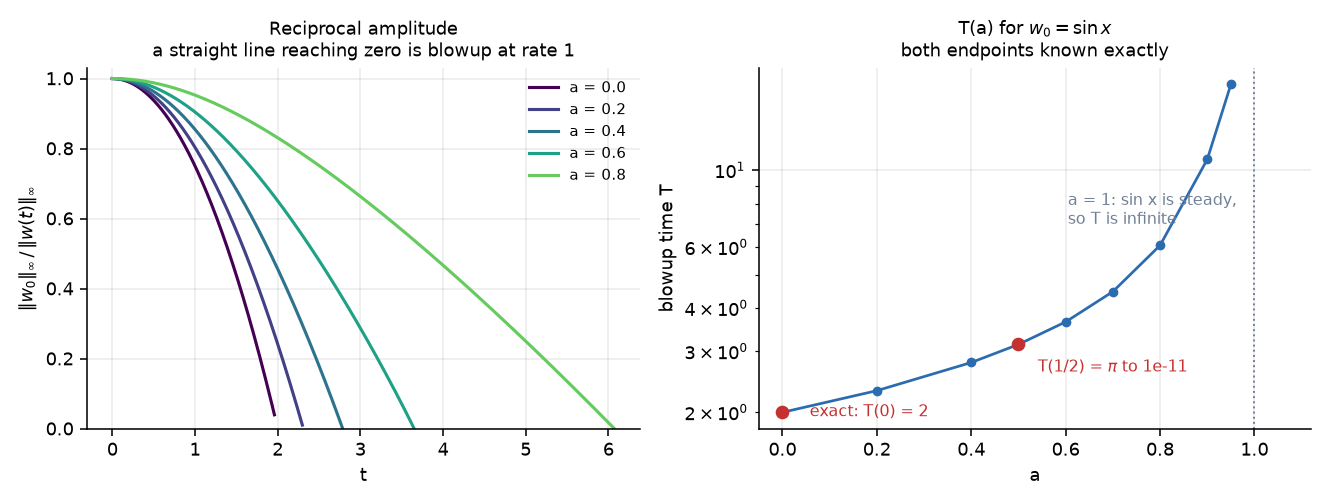
\includegraphics[width=\textwidth]{fig_blowup.png}
\caption{Left: reciprocal amplitude
$\norm{\omega_0}_\infty/\norm{\omega(t)}_\infty$ for several values of $a$. A
straight line reaching zero is blowup with rate exponent one. Right: the
blowup time $T(a)$ from $\omega_0 = \sin x$, on a logarithmic scale. Both
endpoints are known exactly, $T(0)=2$ and $T(1)=\infty$, and the curve runs
between them without any transition to global existence at intermediate $a$.
The agreement of $T(1/2)$ with $\pi$ is marked but unexplained.}
\label{fig:blowup}
\end{figure}

\begin{remark}
The value at $a=1/2$ agrees with $\pi$ to $1.2\times10^{-11}$ and continues to
do so under refinement across an eightfold range in $N$. We have no explanation
for this and record it as an observation.
\end{remark}

The blowups are not all alike. Comparing normalised spectra
$\abs{\hat\omega_k}/\max_k\abs{\hat\omega_k}$ at successive decades of amplitude
growth gives a diagnostic which is invariant under translation and assumes
nothing about the profile shape. At $a=0.8$ the curves converge: successive
deviations from the first snapshot are $3.30\times10^{-3}$,
$3.68\times10^{-3}$, $3.76\times10^{-3}$, $3.78\times10^{-3}$ across four
decades of growth, the peak location locks to $x=2.16699$, and the spectral
tail remains at $2.7\times10^{-17}$ throughout, so a grid of $4096$ points
carries an amplitude of $10^6$ without strain. At $a=0.4$ the same comparison
moves by $0.72$ over a single decade and resolution is exhausted by
$\norm{\omega}_\infty = 5.8\times 10^3$.

\begin{figure}[htbp]
\centering
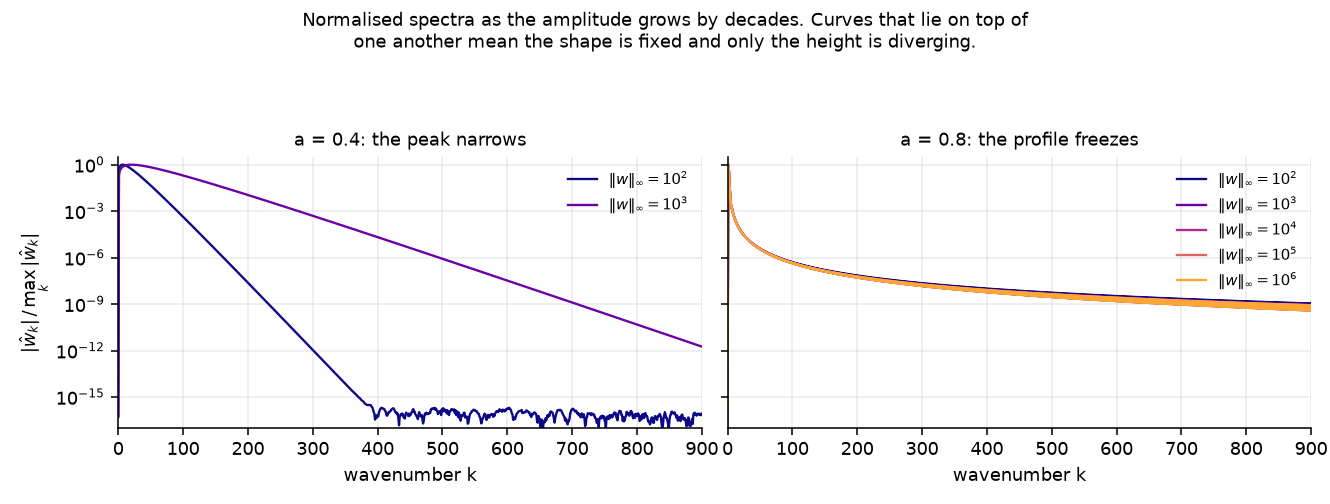
\includegraphics[width=\textwidth]{fig_frozen.png}
\caption{Normalised spectra
$\abs{\hat\omega_k}/\max_k\abs{\hat\omega_k}$ at successive decades of
amplitude growth. Taking the modulus removes the translation, so no alignment
of the peaks is required and the comparison assumes nothing about the profile
shape. Left, $a=0.4$: the curves spread steadily as the peak narrows, and
resolution is exhausted by $\norm{\omega}_\infty = 5.8\times10^3$. Right,
$a=0.8$: five curves spanning four decades of growth lie on top of one
another, so the shape is fixed and only the height diverges.}
\label{fig:frozen}
\end{figure}

We refer to the first behaviour as a \emph{frozen} profile and the second as
\emph{narrowing}, illustrated in Figure \ref{fig:frozen}. Only the frozen case
is analysed below.

The dichotomy is due to \cite{lss2020}, who established it on the circle,
located the transition at $a_c = 0.6890665337007457\ldots$, and computed the
width exponent to five to eight digits by a nonlinear eigenvalue solve. What
this section reports is an independent measurement of the same quantity by a
different and much cruder route, and it should be read as a check on our
diagnostic rather than as a determination of theirs.

The distinction is quantitative. In the general self similar ansatz of
Proposition \ref{prop:general}, the peak width scales like $(T-t)^{c_l}$ while
the amplitude
grows like $(T-t)^{-1}$, so $\text{width}\sim\text{amplitude}^{-c_l}$ and $c_l$
is minus the slope of one against the other on logarithmic axes. A frozen
profile is exactly $c_l=0$. Measuring the width as the half width at half
maximum around the peak, which is robust whether the spectrum is exponential or
algebraic, gives Table \ref{tab:cl}. The method is calibrated at $a=0$, where
the exact solution \eqref{eq:clmexact} has width proportional to $(2-t)$ and
amplitude $4/(4-t^2)$, so $c_l=1$; the measurement returns $1.048$. Against the
published branch, Table \ref{tab:cl} is accurate to a few percent and not of
one sign; the introduction gives that comparison term by term, together with
the estimate of $a_c$ it forces us to withdraw.

\begin{table}[htbp]
\centering
\begin{tabular}{lccccc}
\toprule
$a$ & $0$ & $0.2$ & $0.4$ & $0.5$ & $0.6$\\
$c_l$ & $1.058$ & $0.748$ & $0.512$ & $0.325$ & $0.179$\\
\midrule
$a$ & $0.70$ & $0.74$ & $0.75$ & $0.77$ & $0.80$\\
$c_l$ & $0.032321$ & $0.007273$ & $0.004536$ & $0.001294$ & $0.000398$\\
std.\ err. & $1.5\times10^{-3}$ & $7.5\times10^{-4}$ & $5.4\times10^{-4}$
      & $3.0\times10^{-4}$ & $1.2\times10^{-4}$\\
\bottomrule
\end{tabular}
\caption{The spatial scaling exponent measured from the dynamics. The exact
value at $a=0$ is $1$. The upper block is resolution limited and quoted to two
figures; the lower block is fitted over three decades of amplitude, to $10^6$.
Values at $a\ge 0.78$ are omitted because they are not monotone in $a$ at the
$5\times10^{-4}$ level, which is the true noise floor rather than the smaller
figure the regression reports.}
\label{tab:cl}
\end{table}

\begin{remark}[One signed data]
\label{rem:onesigned}
Lei, Liu and Ren \cite{llr2020} proved global regularity on the circle for data
of one sign at $a=1$. The mechanism appears to reach well below that. From
$\omega_0 = 1-\cos x$, integrating to $t=200$, the amplitude remains bounded at
$2.72$, $2.40$ and $2.17$ for $a=0.7$, $0.8$ and $0.9$, while for $a=0.6$ the
solution reaches $10^6$ by $t=133$ and for $a=0.5$ it exhausts resolution at
$9.6\times10^3$. The threshold lies between $0.6$ and $0.7$. We record this as
an observation; it says nothing about the frozen profile, which is reached from
sign changing data.
\end{remark}

\section{The profile equation}
\label{sec:profile}

Substituting the ansatz
\begin{equation}
  \omega(x,t) = \frac{f(x-x_p)}{T-t}
  \label{eq:ansatz}
\end{equation}
into \eqref{eq:osw} gives $f/(T-t)^2$ on the left and
$\mathcal{R}(f)/(T-t)^2$ on the right, where
\begin{equation}
  \mathcal{R}(f) = f\,\Hil f - a\,U f', \qquad U' = \Hil f,
  \quad \textstyle\int U = 0
\end{equation}
is the same quadratic nonlinearity that drives the evolution. The profile
equation is therefore the fixed point problem
\begin{equation}
  \boxed{\;\mathcal{R}(f) = f.\;}
  \label{eq:profile}
\end{equation}

\begin{proposition}[No free scaling]
\label{prop:scaling}
If $f$ solves \eqref{eq:profile} and $c\ne 1$, then $cf$ does not.
\end{proposition}

\begin{proof}
$\mathcal{R}$ is quadratic, so $\mathcal{R}(cf) = c^2\mathcal{R}(f) = c^2 f$,
which equals $cf$ only when $c^2 f = cf$, that is $c=1$.
\end{proof}

Proposition \ref{prop:scaling} is what makes \eqref{eq:profile} useful rather
than merely descriptive: unlike a linear eigenvalue problem it fixes the
amplitude of $f$ outright. Since \eqref{eq:ansatz} gives
$\norm{\omega(t)}_\infty = \norm{f}_\infty/(T-t)$, we obtain the falsifiable
prediction
\begin{equation}
  \frac{\mathrm{d}}{\mathrm{d}t}\frac{1}{\norm{\omega}_\infty}
  = -\frac{1}{\norm{f}_\infty}.
  \label{eq:rate}
\end{equation}
The left side is measured by time marching the partial differential equation;
the right side by Newton's method on an algebraic fixed point. The two share
nothing but the value of $a$.

We solve \eqref{eq:profile} by Newton iteration, assembling the Jacobian one
column at a time through the same masked transforms used to evaluate
$\mathcal{R}$, and regularising the translation mode by a rank one shift along
$f'$. At $a=0.8$ the profile taken directly from the simulation satisfies
\eqref{eq:profile} to $1.3\times10^{-5}$ before Newton is applied; the
iteration then converges quadratically, with residuals $1.35\times10^{-5}$,
$4.07\times10^{-11}$, $1.77\times10^{-12}$. Table \ref{tab:amp} compares the
two sides of \eqref{eq:rate}.

\begin{table}[htbp]
\centering
\begin{tabular}{lccc}
\toprule
$N$ & simulation, via \eqref{eq:rate} & profile equation & agreement\\
\midrule
$2048$ & $4.148459148$ & $4.148481857$ & $5.5\times10^{-6}$\\
$4096$ & $4.154779433$ & $4.154737187$ & $1.0\times10^{-5}$\\
\bottomrule
\end{tabular}
\caption{$\norm{f}_\infty$ at $a=0.8$, computed two independent ways.}
\label{tab:amp}
\end{table}

\begin{figure}[htbp]
\centering
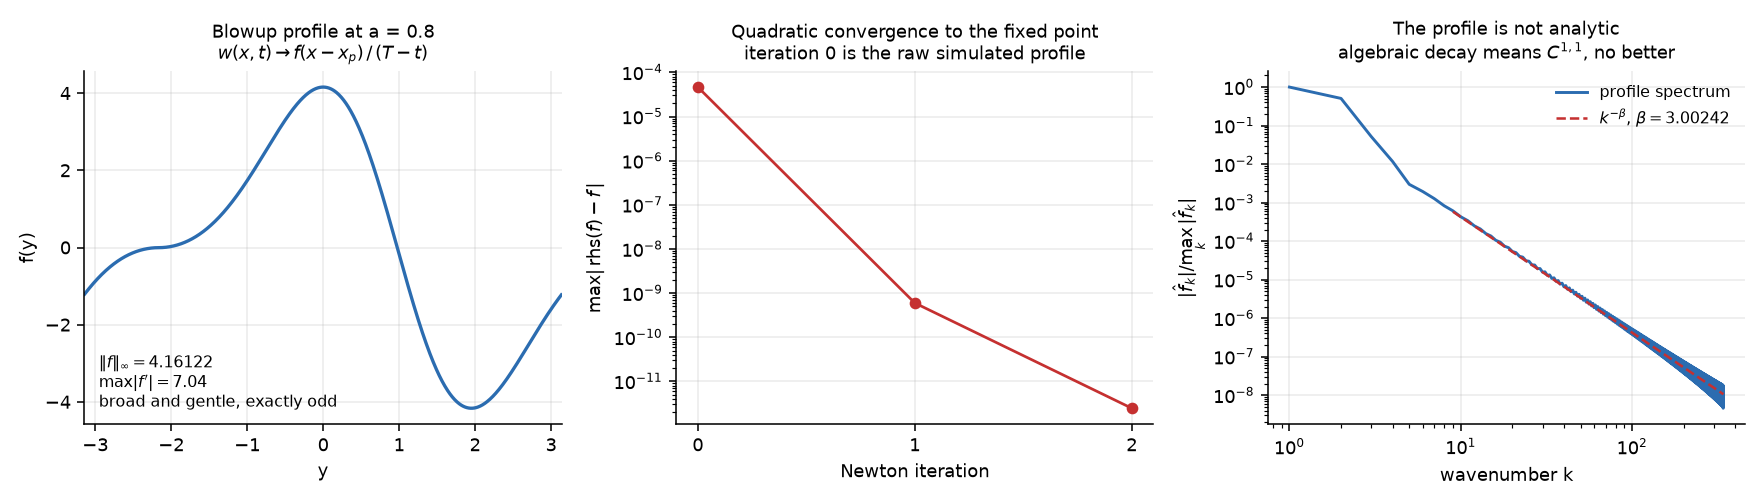
\includegraphics[width=\textwidth]{fig_profile.png}
\caption{The blowup profile at $a=0.8$. Left: $f(y)$, broad and gentle, with
$\norm{f}_\infty = 4.16$ against $\max\abs{f'} = 7.04$, and exactly odd about
each stagnation point. Centre: the Newton residual for \eqref{eq:profile},
starting from the profile taken directly out of the simulation, which already
satisfies the equation to $1.3\times10^{-5}$; convergence is quadratic.
Right: the profile spectrum on logarithmic axes against
$k^{-\beta}$ with $\beta = 3.00242$ from \eqref{eq:beta}, the exponent
predicted in Section \ref{sec:control} rather than fitted to this curve. The
decay is algebraic, not exponential, so the profile is not analytic.}
\label{fig:profile}
\end{figure}

The shared value drifts by $1.5\times10^{-3}$ between the two resolutions,
which is not Newton finding different branches: re-solving at $N=4096$ from the
interpolated $N=2048$ solution returns the same answer, and mapping it back
down reproduces the $N=2048$ value to $2\times10^{-12}$. Each grid has one
solution and the simulation finds that grid's solution. The slow convergence is
explained in Section \ref{sec:stagnation}: the profile is only $C^{1,1}$.

\begin{proposition}[Dilation]
\label{prop:dilation}
If $f$ solves \eqref{eq:profile} then so does $f(n\,\cdot\,)$ for every positive
integer $n$, with the same $\norm{f}_\infty$.
\end{proposition}

\begin{proof}
The Hilbert transform commutes with integer dilation on the circle, so
$\Hil[f(n\,\cdot\,)](x) = (\Hil f)(nx)$. Since the velocity is recovered by
integrating $U' = \Hil f$, the velocity of $f(n\,\cdot\,)$ is $U(nx)/n$, while
$\frac{\mathrm{d}}{\mathrm{d}x}f(nx) = nf'(nx)$. The two factors of $n$ cancel
in the advection term, so
\[
  \mathcal{R}\bigl(f(n\,\cdot\,)\bigr)(x)
  = f(nx)(\Hil f)(nx) - a\,\tfrac{U(nx)}{n}\,n f'(nx)
  = \bigl[f\,\Hil f - a\,Uf'\bigr](nx) = f(nx). \qedhere
\]
\end{proof}

So profiles come in families. The $n$th member carries $2n$ stagnation points
spaced $\pi/n$, with exponents alternating between the two values of the base
member, and $\norm{f}_\infty$, $c_1$, $c_2$ and $\beta$ are all unchanged.
Numerically, $f(n\,\cdot\,)$ solves \eqref{eq:profile} to $10^{-11}$ for
$n \le 4$, against $2\times 10^{-12}$ for the base profile itself.

\paragraph{Genericity.} Every result here starts from $\omega_0 = \sin x$,
which is the ground state of the $a=1$ model and therefore not a generic datum.
Proposition \ref{prop:forced} and the stability computation of Section
\ref{sec:spectrum} predict that any datum in the basin converges to the same
profile, and this is testable independently of them. At $a=0.8$ and $N=2048$:

\begin{table}[htbp]
\centering
\begin{tabular}{lcccc}
\toprule
datum & $\norm{f}_\infty$ & $c_1$ & $c_2$ & $\beta$\\
\midrule
$\sin x$                              & $4.1484819$ & $4.996663$
                                      & $-1.6580199$ & $3.003911$\\
$\sin x + 0.3\sin 2x$                 & $4.1484819$ & $4.996663$
                                      & $-1.6580199$ & $3.003911$\\
$\sin x + 0.5\cos 2x - 0.2\sin 3x$    & $4.1484819$ & $4.996663$
                                      & $-1.6580199$ & $3.003911$\\
$\sin 3x + 0.4\sin 4x$                & $4.1612203$ & $5.006926$
                                      & $-1.668103$ & $2.999354$\\
\bottomrule
\end{tabular}
\caption{The same profile is reached from every datum tested. The first three
agree to seven digits. The fourth lands on the $n=2$ member of Proposition
\ref{prop:dilation}, which on a grid of $2048$ points is represented as
accurately as the base member on $1024$ points, and indeed reproduces the
$N=1024$ values of Table \ref{tab:c2} exactly.}
\label{tab:generic}
\end{table}

\paragraph{Selection.} Solutions of \eqref{eq:profile} exist over a wider range
of $a$ than the dynamics selects. Starting Newton from each simulation's own
profile and recording the residual \emph{before} the iteration begins gives an
order parameter: it reads $0.33$ to $0.56$ for $a$ between $0.3$ and $0.6$,
then $0.19$, $5.0\times10^{-2}$, $2.6\times10^{-3}$, $1.3\times10^{-5}$ and
$5.5\times10^{-5}$ at $a = 0.65, 0.70, 0.75, 0.80, 0.85$. The frozen regime is
therefore roughly $0.75 \le a \le 0.85$ at the amplitudes reached, degrading
smoothly rather than switching off.

\section{The basin, and a third outcome}
\label{sec:basin}

Since $\mathcal{R}$ is quadratic, replacing $\omega_0$ by $\lambda\omega_0$
rescales time and changes nothing else, so the basin is scale invariant and
only shape matters. Combined with Proposition \ref{prop:dilation}, the question
is which member a datum reaches.

\paragraph{Member one is the generic attractor.} Sixteen random data, modes 1
to 8 with amplitudes falling like $1/k$ and random phases, carrying between 4
and 10 sign changes, all reach member one with
$\norm{f}_\infty = 4.148482$ in every case. The number of sign changes does not
select the member. Higher members are reached only from data with the matching
exact symmetry: $\sin(kx)$ gives member $k$ for $k\le 4$, and since $\sin(kx)$
is $2\pi/k$ periodic it remains in that symmetric subspace, while any generic
perturbation returns the solution to member one.

\paragraph{A topological boundary.} For $\omega_0 = \sin x + m$, which changes
sign for $m<1$ and is one signed at $m=1$, blowup occurs for every $m<1$ with
$\norm{f}_\infty = 4.148482$ throughout and $T$ growing as $6.07$, $10.07$,
$15.52$, $20.28$, $25.88$, $43.81$ at $m=0,0.5,0.8,0.9,0.95,0.99$, and ceases
at $m=1$ exactly, where the sign change degenerates into a touching zero. We
fitted the divergence of $T$ and report no law: neither $-\log(1-m)$ nor
$(1-m)^{-p}$ has stable constants over this range.

\paragraph{A third outcome.} Sign change is not sufficient. For
$\omega_0 = \sin x + c\sin 2x$ the two members compete, and between them lies a
window in which the solution does neither:

\begin{table}[htbp]
\centering
\begin{tabular}{lccccccc}
\toprule
$c$ & $0.46$ & $0.475$ & $0.48$ & $0.50$ & $0.52$ & $0.56$ & $0.58$\\
\midrule
outcome & member 1 & member 1 & member 1 & decay & decay & member 2
        & member 2\\
$T$ & $61.4$ & $90.4$ & $108.2$ & - & - & $54.9$ & $44.0$\\
\bottomrule
\end{tabular}
\caption{$T$ diverges on approach from both sides. Inside the window the
amplitude falls monotonically: at $c=0.5$ it reaches $7.4\times10^{-3}$ by
$t=400$ with $\norm{\omega}_\infty t$ settling on $3.09, 3.03, 2.99, 2.97$, so
the solution decays like $1/t$.}
\label{tab:decay}
\end{table}

The window is open rather than a separatrix, since both $c=0.50$ and $c=0.52$
fail to blow up while $0.48$ and $0.56$ do, so the model admits global decaying
solutions from an open set of sign changing data. The window is narrow, roughly
$0.49<c<0.55$.

Decay like $1/t$ invites the guess that the interior is self similar. If
$\omega \sim g/t$ then $R(g) = -g$, and since $\mathcal{R}$ is quadratic
$\mathcal{R}(-g) = \mathcal{R}(g)$, so $h=-g$ would solve \eqref{eq:profile}:
the attractor would be a profile entered with the opposite sign, of amplitude
$2.95$, matching neither member. Writing $s=\log t$ and $W = t\omega$ gives
$W_s = \mathcal{R}(W)+W$, whose linearisation is $-J$, so such a profile would
have to be strongly unstable as a blowup profile.

It is not so. Two tests refute it. Newton started from $-t\omega$ at $t=400$
returns member 1, with $\norm{f}_\infty = 4.1484819$ and its constants and
spectrum; the guess carried an eight percent residual and was never near a
solution. And integrating to $t=2000$ separates the amplitude from the shape:
the decay exponent converges to $1$ and $\norm{\omega}_\infty t$ to $2.950$,
while the normalised spectrum drifts by $4.7\times10^{-3}$, $1.9\times10^{-2}$,
$4.6\times10^{-2}$ at $t = 400, 1400, 2000$ and the residual of $-t\omega$ grows
from $6\times10^{-2}$ to $4.9$ with its sup norm unchanged. Fine structure is
accumulating at high wavenumber rather than a profile settling.

The decay is therefore asymptotically $1/t$ in amplitude and not self similar
in shape. What organises the interior of the window is not a fixed profile and
we do not identify it. The same mechanism accounts for $c=0.52$ exhausting
resolution at $t=42$ while still decaying.

\section{Linear stability in renormalised time}
\label{sec:spectrum}

Set $s = -\log(T-t)$ and $W(y,s) = (T-t)\,\omega$. Then $\omega = e^s W$ and
$\mathrm{d}s/\mathrm{d}t = e^s$, so $\omega_t = e^{2s}(W + W_s)$, while
$\mathcal{R}$ is quadratic and gives $\mathcal{R}(\omega)=e^{2s}\mathcal{R}(W)$.
The factors cancel and
\begin{equation}
  W_s = \mathcal{R}(W) - W.
  \label{eq:renorm}
\end{equation}
The profile is exactly a fixed point of \eqref{eq:renorm}, and the eigenvalues
of $J = D[\mathcal{R}(\cdot)-\cdot](f)$ are growth rates in renormalised time.

\begin{proposition}[Forced eigenvalues]
\label{prop:forced}
$Jf = f$ and $Jf' = 0$.
\end{proposition}

\begin{proof}
Since $\mathcal{R}$ is quadratic, its derivative satisfies
$D\mathcal{R}(f)f = 2\mathcal{R}(f) = 2f$, so
$Jf = D\mathcal{R}(f)f - f = f$. The second identity is translation
invariance: $\mathcal{R}$ commutes with shifts, so differentiating
$\mathcal{R}(f(\cdot+\epsilon)) = f(\cdot+\epsilon)$ at $\epsilon=0$ gives
$D\mathcal{R}(f)f' = f'$ and hence $Jf'=0$.
\end{proof}

The eigenvalue $1$ is not an instability. It reflects the freedom to shift the
blowup time: replacing $T$ by $T+\epsilon$ gives
$W = f\tau/(\tau+\epsilon)$ with $\tau = T-t$, which to first order is
$f - \epsilon e^s f$ and grows like $e^s$. The eigenvalue $0$ is translation.
Numerically, $\norm{Jf-f}_\infty/\norm{f}_\infty = 1.3\times10^{-12}$ and
$\norm{Jf'}_\infty/\norm{f'}_\infty = 4.0\times10^{-11}$, so Proposition
\ref{prop:forced} also serves as a sharp check on the assembled Jacobian.

Every remaining eigenvalue at $a=0.8$ lies in the open left half plane, at
$N=512$, $1024$ and $2048$ alike. The profile is therefore linearly stable up
to the two symmetry directions, which is the precise sense in which the
dynamics selects it, and is consistent with a simulation from $\sin x$ reaching
it without tuning. The same test applied to profiles taken from simulations at
$a=0.65,0.70,0.75,0.80$ returns stability in every case.

\begin{figure}[htbp]
\centering
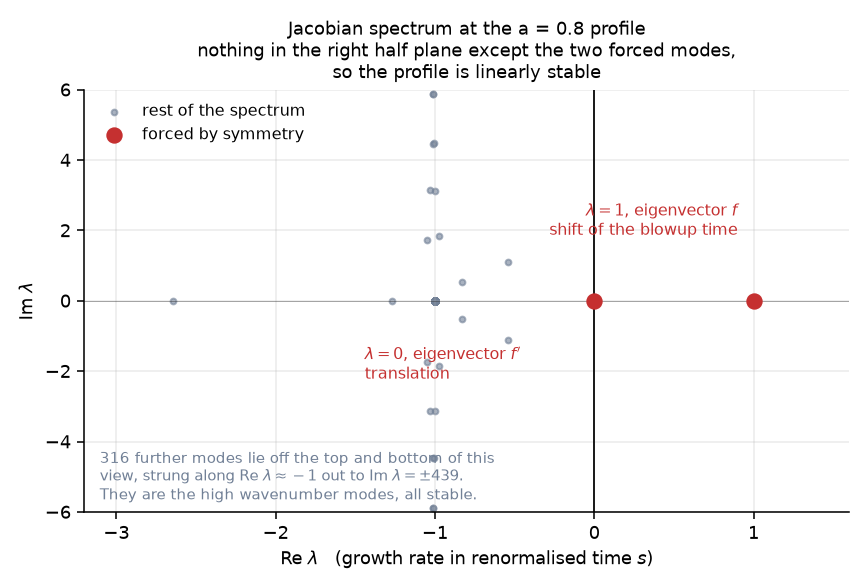
\includegraphics[width=0.72\textwidth]{fig_spectrum.png}
\caption{Spectrum of the linearisation \eqref{eq:renorm} about the $a=0.8$
profile, so that the abscissa is a growth rate in renormalised time $s$. The
two marked eigenvalues are forced by symmetry, at $1$ with eigenvector $f$
(freedom to shift the blowup time) and at $0$ with eigenvector $f'$
(translation), both verified against Proposition \ref{prop:forced} to
$10^{-11}$ or better. Nothing else lies in the closed right half plane. The
modes omitted from the view are the high wavenumber ones, strung along
$\mathrm{Re}\,\lambda \approx -1$ and stable.}
\label{fig:spectrum}
\end{figure}

We note two limitations. The leading stable eigenvalue does not converge in $N$,
taking values $-0.54$, $-0.146$, $-0.41$ at $N=512,1024,2048$, so the rate of
approach to the profile is not determined here, only its sign. At $a=0.85$ and
$N=1024$ the Newton solve lands on a different branch, with
$\norm{f}_\infty = 6.249$ and an unstable eigenvalue at $+2.077$, whereas at
$N=2048$ the same value of $a$ yields $\norm{f}_\infty = 5.668$ matching its
simulation to $8\times10^{-6}$. Continuation in $a$ jumps branches outright.
The branch structure is real and we have not mapped it.

\section{Stagnation points and the local exponent}
\label{sec:stagnation}

This section is background. The relations recalled here are due to
\cite{chenS1} and \cite{xu2026}, and the closed form at a simple zero is a
normalisation identity used throughout this literature. We restate them because
Section \ref{sec:control} rests on them and because the numerics there are
stated in this notation; the proofs are included for self containedness and are
short, not because they are new. Attributions are given after each statement.

Rearranging \eqref{eq:profile} as $a\,U f' = f(\Hil f - 1)$ gives
\begin{equation}
  \frac{f'}{f} = \frac{\Hil f - 1}{a\,U},
  \label{eq:logderiv}
\end{equation}
so $f$ can only be singular where $U$ vanishes.

\begin{proposition}[Local exponent, {\rm \cite{chenS1}}]
\label{prop:exponent}
Let $U(y_\ast)=0$ with $U'(y_\ast)=c\ne 0$. Then $f(y_\ast)=0$, and
$f \sim C\,(y-y_\ast)^{\mu}$ with
\begin{equation}
  \mu = \frac{c-1}{a\,c}.
  \label{eq:mu}
\end{equation}
\end{proposition}

\begin{proof}
Evaluating $a\,Uf' = f(\Hil f - 1)$ at $y_\ast$ gives
$0 = f(y_\ast)\,(c-1)$, so $f(y_\ast)=0$ unless $c=1$. Expanding
$U(y) = c\,(y-y_\ast) + O((y-y_\ast)^2)$ and using $U'=\Hil f$, so that
$\Hil f(y_\ast) = c$, equation \eqref{eq:logderiv} becomes
$f'/f = \mu/(y-y_\ast) + O(1)$ with $\mu$ as stated, and integrating gives the
claim.
\end{proof}

Equation \eqref{eq:mu} is Theorem 1 of \cite{chenS1}. He states it as
$\alpha(a) = \bigl(c_\omega + (1-a)\Hil\omega_a(\pi)\bigr)/\bigl(a\,
\Hil\omega_a(\pi)\bigr)$, where $\alpha$ is the H\"{o}lder exponent of the
\emph{derivative} of the profile at the singular stagnation point, so the
exponent of the profile itself is $1+\alpha$; putting $c_\omega=-1$ and
$\Hil\omega_a(\pi)=c$ gives
$1+\alpha = (ac - 1 + c - ac)/(ac) = (c-1)/(ac)$, which is \eqref{eq:mu}. He
also proves in the same theorem that the profile is $C^1$ but not
$C^{1,\alpha}$ there, which is the regularity statement of this section, and
that the frozen profile exists and is nonlinearly stable for $a$ near $1$. We
obtained \eqref{eq:mu} independently and before finding \cite{chenS1}; the
result is his.

The same computation applies to a narrowing profile. Since the narrowing regime
is where most of this family lives, and since it is the case that can be tested
against an exact solution, we state it in full rather than as an aside.

\begin{proposition}[Local exponent, general self similar form]
\label{prop:general}
Let $\omega = (T-t)^{c_\omega}\Ob\big(x/(T-t)^{c_l}\big)$, so that the profile
equation is
\begin{equation}
  (c_l X + a\,\Ub)\,\Ob_X = (c_\omega + \Ub_X)\,\Ob ,
  \label{eq:profgeneral}
\end{equation}
and let $X_\ast$ be a zero of the total advection velocity $c_l X + a\Ub$,
which replaces $\Ub$ as the transported quantity. Write
$h = \Hil\Ob(X_\ast) = \Ub_X(X_\ast)$ and suppose $c_l + a\,h \ne 0$. Then
$\Ob(X_\ast)=0$ unless $h = -c_\omega$, and $\Ob \sim C\,(X-X_\ast)^{\nu}$ with
\begin{equation}
  \nu = \frac{c_\omega + h}{c_l + a\,h}.
  \label{eq:nugeneral}
\end{equation}
If in addition the zero is simple, that is $\nu = 1$, then
\begin{equation}
  h = \frac{c_l - c_\omega}{1-a},
  \label{eq:hgeneral}
\end{equation}
which for $c_\omega = -1$ reads $h = (1+c_l)/(1-a)$.
\end{proposition}

\begin{proof}
Evaluating \eqref{eq:profgeneral} at $X_\ast$ annihilates the left hand side,
leaving $0 = (c_\omega + h)\,\Ob(X_\ast)$, so $\Ob(X_\ast)=0$ unless
$h = -c_\omega$. Differentiating the advection velocity gives
$(c_l X + a\Ub)_X = c_l + a\,\Ub_X$, which equals $c_l + a\,h$ at $X_\ast$, so
$c_l X + a\Ub \sim (c_l + a\,h)(X-X_\ast)$ there. Dividing
\eqref{eq:profgeneral} by $\Ob$ and by the advection velocity gives
$\Ob_X/\Ob = \nu/(X-X_\ast) + O(1)$ with $\nu$ as stated, and integrating gives
the claim. For \eqref{eq:hgeneral}, setting $\nu=1$ in \eqref{eq:nugeneral}
gives $c_\omega + h = c_l + a\,h$, that is $h(1-a) = c_l - c_\omega$.
\end{proof}

Proposition \ref{prop:exponent} is the case $c_l = 0$, $c_\omega = -1$, which is
what a frozen profile requires: no spatial rescaling, and Proposition
\ref{prop:c1} below is the same case of \eqref{eq:hgeneral}.

Equation \eqref{eq:hgeneral} is not new. \cite{xu2026} derives
$\Hil\Omega(0) = (1+c_l)/(1-a)$ by the same argument, differentiating the
profile equation at the stagnation point under the same nondegeneracy
$\Omega'(0)\ne0$, and records the slope $c_l + a\,\Hil\Omega(0)$ used in the
proof above; we obtained it independently and state it here only because
Proposition \ref{prop:exponent} is the case it does not cover. The content
that remains with us is the exponent at a stagnation point where the zero is
\emph{not} simple, which is the situation at the second stagnation point on the
circle and the one that fixes the spectral decay in
Section \ref{sec:control}. Section \ref{sec:exacthalf} checks the $c_l$
dependence where $c_l\ne0$ and the answer is known exactly.

Since $\abs{y}^\mu$ has Fourier coefficients decaying like $k^{-(\mu+1)}$, the
spectral decay exponent of the profile is
\begin{equation}
  \beta = 1 + \frac{c-1}{a\,c}.
  \label{eq:beta}
\end{equation}
One local number therefore predicts the entire spectral decay rate.

\begin{proposition}[Exact value at a simple zero]
\label{prop:c1}
If in addition $f$ has a simple zero at $y_\ast$, that is $f'(y_\ast)\ne 0$,
then
\begin{equation}
  c = \frac{1}{1-a}.
  \label{eq:c1}
\end{equation}
\end{proposition}

\begin{proof}
Write $f \sim A(y-y_\ast)$ with $A = f'(y_\ast)\ne 0$, $U \sim c(y-y_\ast)$ and
$\Hil f \sim c$. Matching the coefficient of $(y-y_\ast)$ in
$a\,Uf' = f(\Hil f - 1)$ gives $a\,c\,A = A\,(c-1)$, and dividing by $A$ yields
$ac = c-1$, that is $c=1/(1-a)$.
\end{proof}

This identity is standard in this literature, where it is generally used as a
normalisation rather than derived. \cite{chenS1} imposes
$c_\omega(t) = (a-1)u_x(t,0)$ as the gauge fixing the time rescaling, which at
$c_\omega=-1$ is \eqref{eq:c1}; \cite{htw2026} states the general form as
$c_l = c_\omega + (1-a)U_X(0)$ in its equation (2.10); \cite{xu2026} states it
as $\Hil\Omega(0)=(1+c_l)/(1-a)$; and Theorem 1 of \cite{lss2020} reaches
$\gamma = 1/(1-a)$ for the complex singularity exponent from the same balance
$a\gamma = \gamma-1$. We claim none of it. What matters here is only that $c$
at this stagnation point is known in closed form, which is what makes the
control variate of Section \ref{sec:control} possible.

Equivalently $\mu = 1$ at such a point. Numerically, at $N=4096$, the measured
deviation of $\mu$ from $1$ is $-1.7\times10^{-15}$, $-4.6\times10^{-14}$,
$-2.0\times10^{-10}$ and $3.5\times10^{-8}$ at $a=0.70,0.72,0.74,0.76$. The
growth of this deviation at larger $a$ tracks the profile's own accuracy, which
degrades as the second exponent falls toward one. That the identity holds to
machine precision on the discrete profile is what the control variate exploits.

\paragraph{Two stagnation points, exactly $\pi$ apart.} Numerically $U$ has
exactly two zeros, shown with the profile in Figure \ref{fig:beta}, and their
separation is $\pi$ to within $9\times10^{-16}$ for every $a$ tested. This
needs no argument beyond the symmetry of the initial datum. Oddness is
preserved by \eqref{eq:osw}: if $\omega$ is odd about a point then $\Hil\omega$
is even about it, hence $u$ is odd about it, hence both $u\omega_x$ and
$u_x\omega$ are odd about it. Our datum $\omega_0=\sin x$ is odd about $0$ and
about $\pi$, so the solution is odd about both for all time, so $U$ vanishes at
both for all time, and two points antipodal on the circle are $\pi$ apart. The
profile inherits this: scanning for a point about which $f$ is odd, by
minimising $\norm{\mathrm{Re}[\hat f_k e^{iky_0}]}/\norm{\hat f_k}$, returns a
residual of $1.4\times10^{-13}$ at $a=0.8$ located at $y_0=0.975612$, which is
$y_1$ itself, and $10^{-13}$ or smaller at $a=0.75,0.78,0.82$. An earlier
version of this paper gave a Fourier parity argument for the $\pi$ separation
and checked that $f$ does not have only odd modes, $\abs{\hat f_2}=3315$
against $\abs{\hat f_1}=6520$. That check is beside the point: oddness about a
shifted point is far weaker than having only odd modes, and the profile has it.
The construction of \cite{chenS1} takes the profile odd from the outset.

\paragraph{Regularity of the profile.} At $a=0.8$ the second stagnation point
has $\mu \approx 2$, and the general solution of \eqref{eq:logderiv} near a
regular singular point permits different constants on the two sides. We find
$f'' $ bounded and exactly odd about $y_2$ to $10^{-9}$, equal to $+2.27045$ on
one side and $-2.27045$ on the other, a jump of $4.54089$ with
$C_+ = -C_- = 1.13522$. The profile is therefore $C^{1,1}$ but not $C^2$. It is
not a logarithm: fitting $f'' = 2D\log\abs{y-y_2} + \text{const}$ returns a
slope of $0.043$ at $R^2=0.46$, consistent with zero. Correspondingly $f'$ is
continuous at both stagnation points, to $4\times10^{-12}$ and
$1.6\times10^{-11}$.

\section{An exact test at \texorpdfstring{$a=1/2$}{a = 1/2}}
\label{sec:exacthalf}

Every measurement reported above was taken on a frozen profile, where $c_l=0$
and \eqref{eq:nugeneral} cannot be told apart from \eqref{eq:mu}. This section
checks the $c_l$ dependence directly, because \eqref{eq:osw} is solvable in
closed form at $a=1/2$. Nothing in the section is claimed as new: the exact
solution is from \cite{slsa2025}, the exponent $c_l = 1/3$ at $a=1/2$ is stated
in \cite{lss2020} and again in \cite{slsa2025}, and \eqref{eq:hgeneral} is from
\cite{xu2026}. It is included because the three fit together into a
consistency check which is exact rather than numerical, and because the blowup
time it produces for our datum does not appear in any of them.

Silantyev, Lushnikov, Siegel and Ambrose \cite{slsa2025} construct exact pole
dynamics solutions of \eqref{eq:osw} on the circle for $a=0$ and $a=1/2$. In
the variable $X=\tan(x/2)$, which maps $(-\pi,\pi)$ onto $\Real$, their $a=1/2$
solution is a conjugate pair consisting of one double and one simple pole,
whose amplitudes are tied by
$\omega_{-1} = 2iv\,\omega_{-2}/(1-v^2)$; that constraint is what cancels the
logarithmic singularities which advection otherwise generates out of poles. The
initial datum used throughout this paper lies in their class, since partial
fractions give
\begin{equation}
  \sin x \;=\; \frac{2X}{1+X^2} \;=\; \frac{1}{X-i}+\frac{1}{X+i},
  \label{eq:sinpoles}
\end{equation}
a single conjugate pair at $v=1$. That is the limit in which the complex
singularity sits at infinite height, as it must for an entire datum, and it is
the one point at which their parametrisation degenerates: the constraint reads
$1 = (2i/0)\cdot 0$ there. The degeneracy is removable, and clearing it gives
the following, which is a specialisation of \cite{slsa2025} rather than a new
solution.

\begin{proposition}[Blowup time at $a=1/2$]
\label{prop:pi}
For $a=1/2$ and $\omega_0 = \sin x$, the solution of \eqref{eq:osw} blows up at
\begin{equation}
  T \;=\; \pi
  \label{eq:Tpi}
\end{equation}
exactly, with the complex singularity reaching the real axis at $x=\pm\pi$.
\end{proposition}

\begin{proof}
The constraint forces $\omega_{-2,i}(0) = (v^2(0)-1)/(2v(0))$, and substituting
this into the coefficient of the pole equation of \cite{slsa2025} cancels the
vanishing denominator against the vanishing amplitude, leaving
$K = 1/[2(v^2(0)+1)^2]$, which is finite and equal to $1/8$ at $v(0)=1$. The
pole position therefore satisfies the regular equation
\begin{equation}
  \frac{dv}{dt} = \frac{(v^2+1)^3}{32\,v^2},\qquad v(0)=1 .
  \label{eq:poleode}
\end{equation}
Set $G(v) = v(v^2-1)/(v^2+1)^2 + \arctan v$, so that
$G'(v) = 8v^2/(v^2+1)^3$ and \eqref{eq:poleode} integrates to
$G(v(t)) = G(1) + t/4$. The right hand side of \eqref{eq:poleode} is positive,
so $v$ increases and blowup occurs as $v\to\infty$, which is the pole reaching
the real axis at $x=\pm\pi$. Since $G(1)=\pi/4$ and $G(\infty)=\pi/2$,
$T = 4\big[G(\infty)-G(1)\big] = \pi$.
\end{proof}

Taking $v\to\infty$ in the closed form near $x=\pi$, with $z = x-\pi$ and
$\zeta = vz/2$, and using $dv/dt \sim v^4/32$ so that $v^3 = 32/(3(T-t))$,
yields a self similar profile in the sense of Proposition \ref{prop:general}
with
\begin{equation}
  c_l = \tfrac13,\qquad c_\omega = -1,\qquad
  \Ob(\zeta) = -\frac{16}{3}\,\frac{\zeta}{(1+\zeta^2)^2},
  \label{eq:halfprofile}
\end{equation}
whence $\Hil\Ob = -\tfrac83(\zeta^2-1)/(\zeta^2+1)^2$ and
$\Ub = \tfrac83\,\zeta/(\zeta^2+1)$. The value $c_l = 1/3$ is not deduced here
for the first time: it is the exponent $\alpha = 1/3$ recorded at $a=1/2$ in
\cite{lss2020}, where it also arises as the exact value of their approximation
$\alpha_0 = 2/(\gamma(\gamma+1))$ at $\gamma=2$, and it is restated in
\cite{slsa2025} for both of their blowup types. The computation above merely
confirms that our datum sits on the same branch. The total advection velocity
is
\begin{equation}
  c_l\zeta + a\Ub \;=\; \frac{\zeta}{3}\,\frac{\zeta^2+5}{\zeta^2+1},
  \label{eq:halfadv}
\end{equation}
whose only zero is $\zeta=0$, the blowup point itself, and $\Ob$ has a simple
zero there. Proposition \ref{prop:general} then predicts
$h = (1+c_l)/(1-a) = (4/3)/(1/2) = 8/3$, against $1/(1-a) = 2$ for a frozen
profile. The two differ by a third, so the test discriminates.

Measuring $h = (T-t)\,\Hil\omega(\pi,t)$ directly on the exact solution, with
$T-t = 4[G(\infty)-G(v)]$ and the same spectral Hilbert transform used
everywhere else in this paper, gives Table \ref{tab:halfh}. The residual of the
profile equation \eqref{eq:profgeneral} for \eqref{eq:halfprofile} is
$1.3\times10^{-15}$, and $v^3(T-t)\to32/3$ confirms $c_l = 1/3$.

\begin{table}[htbp]
\centering
\begin{tabular}{lccccc}
\toprule
$v$ & $10$ & $30$ & $100$ & $300$ & $1000$\\
\midrule
$h$ measured & $2.671992$ & $2.667259$ & $2.666720$ & $2.666673$ & $2.6666671$\\
$\abs{h - 8/3}$ & $5.3\times10^{-3}$ & $5.9\times10^{-4}$ & $5.3\times10^{-5}$
  & $5.9\times10^{-6}$ & $4.5\times10^{-7}$\\
$\abs{h - 2}$ & $6.7\times10^{-1}$ & $6.7\times10^{-1}$ & $6.7\times10^{-1}$
  & $6.7\times10^{-1}$ & $6.7\times10^{-1}$\\
\bottomrule
\end{tabular}
\caption{The general form of Proposition \ref{prop:general} against the exact
$a=1/2$ solution, at resolutions $N = 2^{14}$ to $2^{20}$. The measurement
converges on $(1+c_l)/(1-a) = 8/3$ and stands off the frozen value
$1/(1-a) = 2$ by two thirds at every resolution.}
\label{tab:halfh}
\end{table}

The same exercise calibrates Table \ref{tab:cl}. That table measures
$c_l = 0.325$ at $a=0.5$ against the exact $1/3$, a shortfall of $2.5$ percent,
while at $a=0$, where $c_l=1$ exactly, it returns $1.048$ to $1.058$. The error
is therefore a few percent and is not of one sign, which is what the fuller
comparison against the published branch in the introduction already showed, and
what makes the withdrawn estimate of $a_c$ untenable.

Finally, $\Ob$ in \eqref{eq:halfprofile} is analytic on $\Real$, its nearest
singularities being at $\zeta = \pm i$. The $C^{1,1}$ regularity and the
algebraic spectral decay \eqref{eq:beta} found in Section \ref{sec:stagnation}
are thus features of the frozen regime specifically, not of blowup in this
family generally. That is consistent with Proposition \ref{prop:general}: with
$c_l>0$ the total advection velocity has a nonzero slope $c_l + a h$ at the
stagnation point even when $\Ub$ alone would vanish to higher order, so the
regular singular point is milder.

\section{Determination of the global constant}
\label{sec:control}

Proposition \ref{prop:c1} pins the stagnation point at which the profile is
smooth, and which therefore contributes no singularity. The exponent $\beta$ is
set by the other one, whose $c$, written $c_2$ below, is genuinely global: no
local balance determines it.

Reading $c_2$ off a single grid is unreliable. Across $N=512$ to $4096$ it
wanders between $-1.6486$ and $-1.6681$ without a monotone trend, and a three
parameter fit of the form $c_2(N) = c_2^\infty + AN^{-p}$ returns $p=3.3$ with
amplitude $1.1\times10^7$, which is a fit to noise. The reason is the $C^{1,1}$
regularity established above: every quantity read from the profile converges
algebraically.

The remedy is that $c_1$ is known exactly. Both constants are read from the
same profile and carry the same discretisation error, entering linearly, so
$c_2$ is a linear function of $c_1$ across resolutions and evaluating that line
at the exact $c_1$ cancels the error without requiring its size or its rate. At
$a=0.8$ the regression over seven resolutions is
\begin{equation}
  c_2 = -0.980361\,c_1 + 3.240505, \qquad R^2 = 0.99999744,
\end{equation}
and the raw spread of $1.95\times10^{-2}$ collapses to $2.43\times10^{-5}$, a
factor of $801$. The corrected value from $N=512$ then lies within
$1.5\times10^{-5}$ of that from $N=4096$. We obtain
\begin{equation}
  c_2 = -1.66130027 \pm 1.0\times10^{-5}, \quad
  \mu_2 = 2.00242268, \quad
  \beta = 3.00242268.
\end{equation}

\begin{table}[htbp]
\centering
\begin{tabular}{lcccc}
\toprule
$a$ & $c_2$ & scatter & $\mu_2$ & $\beta$\\
\midrule
$0.70$ & $-0.10252834$ & $4.1\times10^{-16}$ & $15.36200$  & $16.36200$\\
$0.71$ & $-0.20450843$ & $6.0\times10^{-16}$ & $8.29546$   & $9.29546$\\
$0.72$ & $-0.31519119$ & $1.4\times10^{-14}$ & $5.7953854$ & $6.7953854$\\
$0.74$ & $-0.56651088$ & $4.2\times10^{-10}$ & $3.7367448$ & $4.7367448$\\
$0.76$ & $-0.86560395$ & $1.8\times10^{-8}$  & $2.8358720$ & $3.8358720$\\
$0.78$ & $-1.22477889$ & $1.3\times10^{-6}$  & $2.3288127$ & $3.3288127$\\
$0.80$ & $-1.66130509$ & $1.2\times10^{-5}$  & $2.0024205$ & $3.0024205$\\
$0.82$ & $-2.20024724$ & $5.3\times10^{-5}$  & $1.7737736$ & $2.7737736$\\
\bottomrule
\end{tabular}
\caption{The global constant and the resulting exponents. The scatter is the
spread of the corrected values across resolutions and measures self
consistency, not residual systematic error. The rows at $a=0.70$ and $a=0.71$
were computed over $N = 1024$ to $3072$ rather than the full ladder, and are
quoted to the digits that run resolves.}
\label{tab:c2}
\end{table}

\begin{figure}[htbp]
\centering
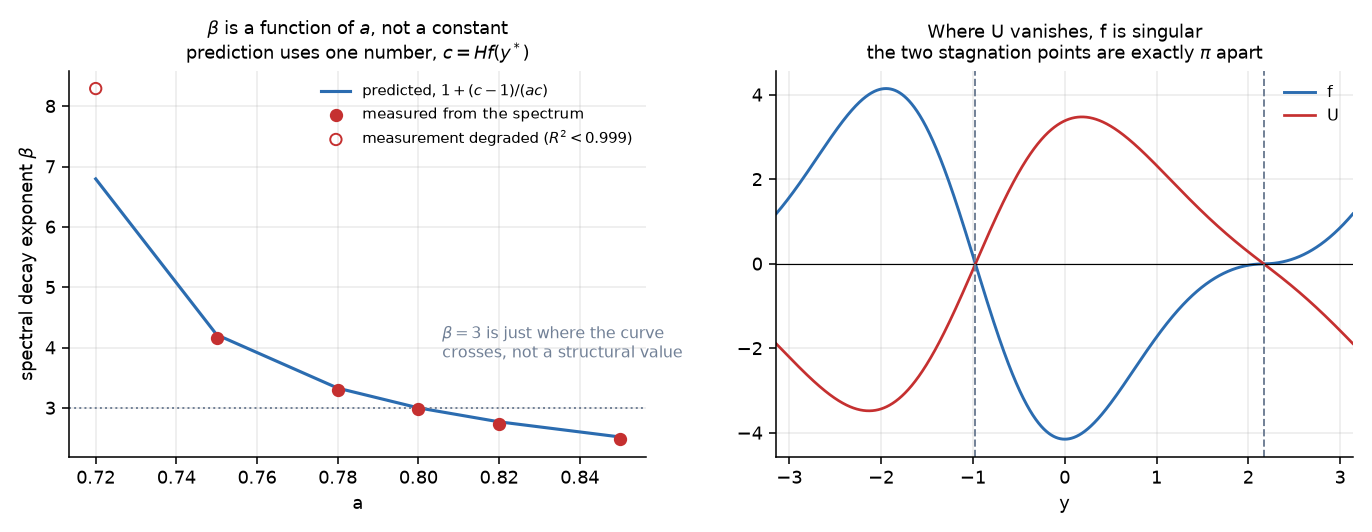
\includegraphics[width=\textwidth]{fig_beta.png}
\caption{Left: the spectral decay exponent $\beta$ against $a$, from
\eqref{eq:beta} with $c_2$ fixed by the control variate. The curve is smooth
and $\beta=3$ is simply where it crosses. Direct fits of
$\abs{\hat f_k}\sim k^{-\beta}$ to the spectrum are shown for contrast with
error bars of $\pm 0.02$, which is their window sensitivity; the relation is
four orders of magnitude more accurate than measuring the exponent directly.
Right: the profile $f$ and its velocity $U$ at $a=0.8$. The dashed lines mark
the two zeros of $U$, which are exactly $\pi$ apart, and $f$ vanishes at both
as Proposition \ref{prop:exponent} requires.}
\label{fig:beta}
\end{figure}

\begin{remark}[$\beta \ne 3$]
The value $\mu_2 = 2$, and hence $\beta=3$, would require
$c_2 = 1/(1-2a) = -1.66666667$ at $a=0.8$. The corrected value misses this by
$5.37\times10^{-3}$, some five hundred times the scatter of the corrected
points. Since the correction removes eight hundred times the raw error, the
conclusion survives allowing a residual systematic an order of magnitude above
the observed scatter. Table \ref{tab:c2} shows $\beta$ varying continuously
with $a$; the value $3$ is merely where that curve crosses.
\end{remark}

\begin{remark}[Against the published exponent]
\label{rem:pb}
\cite{lss2020} measure this same exponent for the frozen profile, calling it
$p_b$, by a two domain least squares fit to the spectrum, and report
$p_b = 9.32592$ at $a=0.71$. Equation \eqref{eq:beta} with $c_2$ from Table
\ref{tab:c2} gives $\beta = 9.29546$ there, lower by $0.03046$, or $0.33$
percent. The two determinations share nothing: theirs is a fit to the tail of
the spectrum over a window, ours is a single value of $\Hil f$ read off the
profile at a point. Given the window sensitivity documented in the next remark
we read the difference as a correction to the fitted value rather than a
disagreement, and we claim no more than the three digits it rests on.

Their exponent diverges as $a\to a_c^+$, and $\beta$ here does the same, which
gives an independent handle on $a_c$. Extrapolating $1/\beta$ linearly to zero
from the pairs $(0.70,0.71)$ and $(0.71,0.72)$ gives $0.6868$ and $0.6828$,
with the pair nearer the transition returning the larger value, pointing at
their $a_c = 0.6890665337007457\ldots$ and not at anything larger. This is an
extrapolation through convex data, so we quote it for its direction only, but
that direction is what withdraws the estimate of $a_c$ discussed in the
introduction.
\end{remark}

\begin{remark}[On measuring $\beta$ from the spectrum directly]
We caution against it. Fitting $\abs{\hat f_k}\sim k^{-\beta}$ over a band is
sensitive to the band at the $2\times10^{-2}$ level: shifting the window from
$128 \le k \le 512$ to $0.094\,k_{\mathrm{cut}} \le k \le
0.375\,k_{\mathrm{cut}}$, the same window to three digits, moves the answer
from $3.00315$ to $2.98626$. Across ten reasonable windows a binned estimator
spans $2.9829$ to $3.0072$ and an unbinned least squares fit spans $3.0132$ to
$3.0510$, and the two barely overlap. The two ends of the spectrum are biased
in opposite directions: the low end by the analytic factor multiplying
$\abs{y-y_\ast}^\mu$, which contributes $k^{-(\mu+2)}$ and faster, and the high
end by the dealiasing mask. Refinement distinguishes them, since the former is
pinned to absolute $k$ and the latter to a fixed fraction of
$k_{\mathrm{cut}}$. Equation \eqref{eq:beta} with a well determined $c_2$ is
four orders of magnitude more accurate than any of these fits.
\end{remark}

\section{A first integral and a global constraint}
\label{sec:integral}

Equation \eqref{eq:logderiv} integrates in closed form. On any interval free of
zeros of $U$,
\begin{equation}
  f = C\,\abs{U}^{1/a}\exp\Bigl(-\frac1a\int \frac{\mathrm{d}y}{U}\Bigr).
  \label{eq:firstintegral}
\end{equation}
Near a simple zero this yields
$\abs{y-y_\ast}^{1/a}\abs{y-y_\ast}^{-1/(ac)} = \abs{y-y_\ast}^{\mu}$,
recovering Proposition \ref{prop:exponent} independently.

\begin{proposition}[Global constraint]
\label{prop:pv}
If $f$ and $U$ are $2\pi$ periodic and $\log\abs{f}$ has no jump at either
zero of $U$, then
\begin{equation}
  \mathrm{PV}\oint \frac{\mathrm{d}y}{U} = 0.
  \label{eq:pv}
\end{equation}
\end{proposition}

\begin{proof}
Integrating \eqref{eq:logderiv} once around the circle,
$0 = \frac1a\bigl[0 - \mathrm{PV}\oint \mathrm{d}y/U\bigr]$, since both
$\log\abs{f}$ and $\log\abs{U}$ return to their initial values.
\end{proof}

The hypothesis holds here: at $y_1$ the profile is smooth with $\mu=1$, and at
$y_2$ the one sided constants satisfy $C_+=-C_-$, so $\abs{C_+}=\abs{C_-}$ and
the logarithm does not jump. We verify \eqref{eq:pv} by subtracting both simple
poles with $\cot$, which carries the same residue and whose own principal value
on the circle vanishes. The resulting ratios are $2.2\times10^{-12}$,
$6.7\times10^{-13}$, $9.8\times10^{-13}$ and $1.4\times10^{-12}$ at
$a=0.75,0.78,0.80,0.82$, stable across three independent grid shifts.

\begin{remark}
A naive evaluation of \eqref{eq:pv} on the grid returns ratios between
$10^{-2}$ and $1$ and appears to refute it. This is catastrophic cancellation:
the stagnation points land on grid points to within $10^{-11}$ of a cell, so
the subtraction differences two quantities of size $10^{8}$. Evaluating on a
half shifted grid, which is exact for a band limited field, resolves it.
\end{remark}

\paragraph{No closed form for $c_2$.} With $c_2$ determined across eleven values
of $a$, candidate shapes can be excluded rather than merely left unconfirmed.
Every M\"{o}bius form is rejected: $\mu_2 = (p+qa)/(1+ra)$ leaves an rms
residual of $1.9\times10^{-4}$, $c_2 = (p+qa)/(1+ra)$ leaves
$3.0\times10^{-4}$, and the same shape in the variable $1/(1-a)$ leaves
$6.0\times10^{-4}$, each one to two orders above the data's precision. Fits of
quadratic over quadratic achieve residuals of order $10^{-7}$ but use five
parameters against eleven points and dip below the data scatter at the rough
end of the range, so they absorb smooth error rather than signal and we do not
regard them as evidence.

We suggest this is the correct answer rather than a gap. Proposition
\ref{prop:c1} succeeds because it is a \emph{local} balance at a point where
$f$ is smooth. No such balance is available at the second stagnation point, so
its value is determined by the global solution. Writing $\psi$ for the positive
frequency part of $U$, so that $U = \psi+\bar\psi$ and
$f = i(\psi'-\bar\psi')$, equation \eqref{eq:profile} reads
\begin{equation}
  a\,(\psi+\bar\psi)(\psi''-\bar\psi'')
  = (\psi'-\bar\psi')(\psi'+\bar\psi'-1),
\end{equation}
and the mixed products $\psi\bar\psi''$ and $\bar\psi\psi''$ straddle both
halves of the spectrum. That failure to separate is exactly what makes $a=0$
integrable and $a\ne 0$ not.

\section{The critical limit \texorpdfstring{$a\to 1$}{a to 1}}
\label{sec:critical}

The case $a=1$ is degenerate in a way no other member of the family is.

\begin{proposition}[Line of equilibria]
\label{prop:line}
At $a=1$, every $A\sin x$ with $A\in\Real$ is a steady state of
\eqref{eq:osw}, as is every translate.
\end{proposition}

\begin{proof}
With $\omega = A\sin x$ we have $\Hil\omega = -A\cos x$, $u = -A\sin x$ and
$\omega_x = A\cos x$, so
$\omega\,\Hil\omega = -A^2\sin x\cos x = u\,\omega_x$ and
$\mathcal{R}_1(\omega) = \omega\,\Hil\omega - u\,\omega_x = 0$.
\end{proof}

So the critical case carries a two parameter manifold of equilibria, amplitude
and translation, which exists at $a=1$ and nowhere else. Writing
$\varepsilon = 1-a$, the family is destroyed at order $\varepsilon$ and the
blowup time diverges. We measure $T$ without fitting: for a frozen profile
$\norm{\omega}_\infty = \norm{f}_\infty/(T-t)$ exactly, so
$T = t + \norm{f}_\infty/\norm{\omega}_\infty$ at any late time, and running to
$\norm{\omega}_\infty = 10^6$ makes the correction term of order $10^{-6}$.

\begin{table}[htbp]
\centering
\begin{tabular}{lcccccccc}
\toprule
$a$ & $0.80$ & $0.90$ & $0.93$ & $0.95$ & $0.96$ & $0.97$ & $0.98$ & $0.99$\\
\midrule
$T$ & $6.0719$ & $10.7569$ & $14.0844$ & $17.7129$ & $20.4591$ & $24.5830$
    & $32.1786$ & $56.9742$\\
$T\varepsilon$ & $1.214$ & $1.076$ & $0.986$ & $0.886$ & $0.818$ & $0.737$
    & $0.644$ & $0.570$\\
local $p$ & - & $0.828$ & $0.755$ & $0.681$ & $0.646$ & $0.638$ & $0.664$
    & $0.824$\\
\bottomrule
\end{tabular}
\caption{Blowup time as $a\to1$, and the local exponent in
$T\sim\varepsilon^{-p}$ between consecutive entries. $T\varepsilon$ decreases
throughout, so $T$ grows strictly slower than $1/\varepsilon$, but $p$ does not
converge.}
\label{tab:critical}
\end{table}

The exponent does not settle: it falls from $0.83$ to $0.64$ and returns to
$0.82$ at the smallest $\varepsilon$. No functional form fits the last points,
$C\varepsilon^{-p}$, $C/\varepsilon+D$, $C\log(1/\varepsilon)+D$ and
$A/\varepsilon + B\log(1/\varepsilon)+C$ leaving rms residuals of $0.99$,
$0.71$, $4.22$ and $0.38$ against $T$ values from $6$ to $57$. We therefore
quote no exponent. What follows instead is an account of why the natural
reductions do not settle it either.

\subsection{The two mode reduction is exact, and gives the wrong answer}

Expanding about the manifold, put $\omega = A\sin x + B\sin 2x$. Using
$\Hil\sin kx = -\cos kx$ and $u = -k^{-1}\sin kx$,
\begin{align*}
  \omega\,\Hil\omega &= -\tfrac{A^2}{2}\sin 2x - AB\sin 3x
                        - \tfrac{B^2}{2}\sin 4x,\\
  u\,\omega_x        &= -\tfrac{A^2}{2}\sin 2x - \tfrac{5AB}{4}\sin 3x
                        + \tfrac{3AB}{4}\sin x - \tfrac{B^2}{2}\sin 4x,
\end{align*}
so that $\mathcal{R}_a = \omega\,\Hil\omega - a\,u\,\omega_x$ has coefficients
$-\tfrac{3a}{4}AB$ on $\sin x$, $-\tfrac{\varepsilon}{2}A^2$ on $\sin 2x$,
$(\tfrac{5a}{4}-1)AB$ on $\sin 3x$ and $-\tfrac{\varepsilon}{2}B^2$ on
$\sin 4x$, each verified against the solver to $10^{-17}$.

The $\sin x$ terms cancel in the first line but not the second, so the feedback
of mode two into mode one survives at \emph{linear} order. Any argument
predicting $p=2/3$ from a parity cancellation is therefore excluded, not by
numerics but by the calculation.

Retaining the two modes gives $A' = -\tfrac{3a}{4}AB$,
$B' = -\tfrac{\varepsilon}{2}A^2$, which integrates in closed form. Setting
$L=\log A$ at $a=1$ gives $L' = -\tfrac34 B$ and
$L'' = \tfrac{3\varepsilon}{8}e^{2L}$, a Liouville equation; multiplying by
$L'$ and using $L(0)=L'(0)=0$ gives
$L'^2 = \tfrac{3\varepsilon}{8}(e^{2L}-1)$, and since
$\int_0^\infty (e^{2L}-1)^{-1/2}\,\mathrm{d}L = \arccos(e^{-L})\big|_0^\infty
= \pi/2$,
\begin{equation}
  T_{2} = \frac{\pi}{2}\sqrt{\frac{8}{3\varepsilon}}
        = 2.56510\,\varepsilon^{-1/2}.
  \label{eq:liouville}
\end{equation}
Against a two mode Galerkin truncation the ratio $T/T_2$ reads $1.118$,
$1.054$, $1.026$, $1.010$, $1.005$ at
$\varepsilon = 0.2, 0.1, 0.05, 0.02, 0.01$. The reduction is exact and gives
$p = 1/2$, which is not the behaviour of the full equation.

\subsection{The exponent is carried by the cascade}

Retaining $m$ modes and measuring the exponent over
$0.02\le\varepsilon\le0.1$ gives the following.

\begin{table}[htbp]
\centering
\begin{tabular}{lcccccc}
\toprule
$m$ & $2$ & $4$ & $6$ & $8$ & $12$ & $24$\\
\midrule
$p$ & $0.474$ & $0.506$ & $0.518$ & $0.525$ & $0.536$ & $0.554$\\
\bottomrule
\end{tabular}
\caption{Exponent from an $m$ mode Galerkin truncation. The value climbs
monotonically and is still climbing at $m=24$; at $\varepsilon=0.1$ the gap to
the full answer closes like $m^{-1/2}$.}
\label{tab:trunc}
\end{table}

No finite truncation reproduces the exponent. The case $m=3$ is degenerate and
sits outside the trend, giving $T=405$ at $\varepsilon=0.1$ and no blowup at
all at $0.05$ or $0.02$.

\subsection{There is no spectral gap, hence no reduction}

Both failures have one cause. Since $\mathcal{R}$ is quadratic,
$D\mathcal{R}_1(A\sin x) = A\,M$ with $M = D\mathcal{R}_1(\sin x)$ independent
of $A$, and writing $\omega = A\sin x + v$,
\begin{equation}
  v_t = A\,Mv - \tfrac{\varepsilon}{2}A^2\sin 2x,
  \qquad A' = -\tfrac{3}{4}A\,b_2,
  \label{eq:escape}
\end{equation}
with $b_2$ the $\sin 2x$ component of $v$. Were $M$ strictly stable, $v$ would
saturate at $\tfrac{\varepsilon}{2}AM^{-1}\sin 2x$ and \eqref{eq:escape} would
reduce to $A' = \kappa\varepsilon A^2$, a Riccati equation giving $p=1$. That
step is unavailable.

\begin{observation}[No gap]
\label{obs:gap}
The spectrum of $M$ is purely imaginary. Computed densely at $N=128,256,512$,
every eigenvalue has real part at the $10^{-5}$ roundoff level against
imaginary parts reaching $72$, and at $N=256$ none has positive real part.
Its kernel contains the tangent directions to the manifold exactly:
$\norm{M\sin x}_\infty = 8\times10^{-14}$ and
$\norm{M\cos x}_\infty = 6\times10^{-14}$.
\end{observation}

Moreover $M$ is not diagonalisable. Integrating $v_t = Mv$ from a random
perturbation, $\norm{v}$ grows linearly, by factors $187, 736, 1392, 2873,
5738$ at $t = 10, 50, 100, 200, 400$, doubling as $t$ doubles; with imaginary
spectrum this means a Jordan block at zero. Splitting the state identifies its
origin. The components along $\sin x$ and $\cos x$ grow linearly, reaching
$2663$ and $-845$ at $t=400$, while the remainder stays bounded and oscillates
between $135$ and $467$. The secular growth is therefore \emph{drift along the
manifold of equilibria} rather than instability: a perturbation alters the
amplitude and phase at a constant rate, carrying the state to a different
steady state rather than away from all of them. The Jordan block is generated
by the symmetries themselves, consistent with the stability theorem of Jia,
Stewart and Sverak \cite{jss2019}, which is stability modulo exactly these
symmetries.

We note also that $M$ is strongly non-normal: the remainder above is amplified
from $7.8$ to $467$ before returning, a transient factor near $60$ with no
eigenvalue to account for it.

The consequence is structural. Modulo the kernel every mode oscillates without
decay and the kernel modes drift linearly, so there is no gap anywhere. Hence
quasi steady elimination is invalid, because the transient it discards never
dies; mode truncation is not a reduction, because the discarded modes never
relax, which is why the truncated exponent converges only algebraically; and
there is no centre manifold to reduce onto, because the centre subspace is the
whole space. The cascade cannot be eliminated because nothing within it is fast
relative to anything else, and \eqref{eq:liouville}, exact yet giving the wrong
exponent, is the sharpest available demonstration that a finite reduction
misses the mechanism rather than approximating it.

\section{Limitations}
\label{sec:caveats}

The datum $\sin x$ is not generic: it is precisely the ground state of the
$a=1$ model. Table \ref{tab:generic} and Section \ref{sec:basin} between them
answer the worst form of this objection, reaching the same profile from
sixteen random data, from a continuous family of offsets and from three
designed data, always with the same constants to seven digits.

What remains open is the shape of the basin boundary rather than its
existence. Two one parameter families were probed in a space of functions, and
the decay window of Section \ref{sec:basin} already shows the boundary is not
simply whether the datum changes sign. Nothing here maps it in more than one
dimension, and the interior of the decay window is not resolved: $c=0.52$ goes
under resolved at $t=42$ while still decaying.

All statements about $a=0.9$ and above are unresolved. The residual of the
profile equation there does not fall monotonically with the amplitude cap,
taking values $0.78$, $2.93$, $1.77$ at caps $10^4$, $10^6$, $10^8$, so those
measurements reflect the fitting window rather than the solution. Since
$T(0.9)\approx 10.8$ against $6.1$ at $a=0.8$, comparisons should be made at a
fixed fraction of $T$ rather than a fixed amplitude.

The scatter quoted in Table \ref{tab:c2} measures how consistently the control
variate reproduces itself across resolutions. A residual nonlinear dependence
of the discretisation error on $c_1$ would cancel from it and go undetected, so
the figure of $1.4\times10^{-14}$ at $a=0.72$ should not be read as fourteen
digit accuracy.

On priority. The bibliographic details of every reference above have been
verified. Twelve closely related works have been read for overlap:
\cite{osw2008}, \cite{htw2022}, \cite{hqww2023}, \cite{hqw2024},
\cite{zheng2023}, \cite{gj2025}, \cite{htw2026}, \cite{lss2020},
\cite{slsa2025}, \cite{xu2026}, \cite{chenS1} and \cite{alss2022}. The honest
summary is that this is a numerical note about a constant, in a setting other
people built.

We claim none of the following. The two regime picture on the circle, the
critical advection $a_c$, the frozen blowup $\omega = f(x)/(T-t)$ and its
numerical profile, the derivative jump at the antipodal point, the algebraic
spectral decay it causes, and stability as inferred from converging
simulations, are all in \cite{lss2020}. Existence and nonlinear stability of
the frozen profile for $a$ near $1$, the local exponent \eqref{eq:mu}, and the
$C^1$ but not $C^{1,\alpha}$ regularity at the singular stagnation point are
Theorems 1 and 2 of \cite{chenS1}. Equation \eqref{eq:hgeneral} and hence
Proposition \ref{prop:general} appear in \cite{xu2026} and, as equation (2.10),
in \cite{htw2026}, and Proposition \ref{prop:c1} is the normalisation
\cite{chenS1} imposes to fix the time rescaling. The exact $a=1/2$ solution of
Section \ref{sec:exacthalf} is from \cite{slsa2025}, and Proposition
\ref{prop:pi} is a specialisation of it. We derived several of these relations
independently before finding the references, which is a fact about how the work
went and not a claim on it.

What we claim is the control variate of Section \ref{sec:control} and what it
yields: $\beta$ to five digits, the exclusion of $\beta=3$ at $a=0.8$, and the
correction to the fitted exponent of \cite{lss2020} recorded in Remark
\ref{rem:pb}; the linear spectrum of Section \ref{sec:spectrum} at $a=0.8$,
which is numerical where \cite{chenS1} is a theorem near $a=1$; and the first
integral and global constraint of Section \ref{sec:integral}, which we did not
find in \cite{chenS1}, \cite{htw2026} or the pole dynamics papers, though both
are elementary consequences of separating \eqref{eq:logderiv} and we would not
be surprised to be shown otherwise.

This reference list grew four times while being compiled, and that history is
the strongest caveat we can offer. \cite{lss2020}, \cite{slsa2025},
\cite{xu2026} and \cite{alss2022} belong to a line of work using complex
singularity and pole dynamics methods which searches organised around the other
references do not surface, and it is the line that works on the circle.
\cite{chenS1} was found later still, through a citation inside \cite{alss2022}
which turned out to describe it inaccurately. We have read \cite{lss2020} in
full and \cite{chenS1} and \cite{xu2026} in part, and for the preprints this
rests on a reading of the text rather than a line by line verification of every
lemma. Both numerical coincidences with \cite{htw2026} have been examined;
neither is an overlap, and the first, the exchange of stability near
$a\approx0.75$, is to be compared against $a_c = 0.68907$ rather than against
the estimate withdrawn above, and remains unsettled.

The critical limit is left open. Section \ref{sec:critical} reports no exponent
for $T(\varepsilon)$ because the measured one does not converge over the range
we can reach, and reaching $\varepsilon = 10^{-3}$ would need some thirty times
the $866{,}000$ steps that $\varepsilon = 10^{-2}$ already took. Observation
\ref{obs:gap} explains why the shortfall cannot be made up by analysis in place
of computation, but it is an explanation of a difficulty rather than a
resolution of it.

Finally, nothing here is a proof. A computer assisted proof in this setting, in
the style of Chen and Hou \cite{chenhou2022}, requires interval arithmetic
producing certified enclosures rather than floating point with convergence
studies. The objects this paper produces, a profile equation with a linearly
stable solution and an exact relation fixing one of its two local constants,
are the objects such a proof would need to enclose.

\begin{thebibliography}{99}

\bibitem{clm1985} P. Constantin, P. D. Lax and A. Majda,
  \emph{A simple one dimensional model for the three dimensional vorticity
  equation}, Comm. Pure Appl. Math. \textbf{38} (1985), 715-724.

\bibitem{degregorio1990} S. De Gregorio,
  \emph{On a one dimensional model for the three dimensional vorticity
  equation}, J. Statist. Phys. \textbf{59} (1990), 1251-1263.

\bibitem{osw2008} H. Okamoto, T. Sakajo and M. Wunsch,
  \emph{On a generalization of the Constantin, Lax and Majda equation},
  Nonlinearity \textbf{21} (2008), 2447-2461.

\bibitem{jss2019} H. Jia, S. Stewart and V. \v{S}ver\'{a}k,
  \emph{On the De Gregorio modification of the Constantin, Lax and Majda
  model}, Arch. Ration. Mech. Anal. \textbf{231} (2019), 1269-1304.

\bibitem{llr2020} Z. Lei, J. Liu and X. Ren,
  \emph{On the Constantin, Lax and Majda model with convection},
  Comm. Math. Phys. \textbf{375} (2020), 765-783.

\bibitem{chh2021} J. Chen, T. Y. Hou and D. Huang,
  \emph{On the finite time blowup of the De Gregorio model for the 3D Euler
  equations}, Comm. Pure Appl. Math. \textbf{74} (2021), 1282-1350.

\bibitem{luohou2014} G. Luo and T. Y. Hou,
  \emph{Potentially singular solutions of the 3D axisymmetric Euler
  equations}, Proc. Natl. Acad. Sci. USA \textbf{111} (2014), 12968-12973.

\bibitem{elgindi2021} T. M. Elgindi,
  \emph{Finite time singularity formation for $C^{1,\alpha}$ solutions to the
  incompressible Euler equations on $\Real^3$}, Ann. of Math. \textbf{194}
  (2021), 647-727.

\bibitem{chenhou2022} J. Chen and T. Y. Hou,
  \emph{Stable nearly self similar blowup of the 2D Boussinesq and 3D Euler
  equations with smooth data I: Analysis}, preprint, arXiv:2210.07191 (2022).

\bibitem{chenhou2025} J. Chen and T. Y. Hou,
  \emph{Stable nearly self similar blowup of the 2D Boussinesq and 3D Euler
  equations with smooth data II: Rigorous numerics},
  Multiscale Model. Simul. \textbf{23} (2025), 25-130.

\bibitem{htw2022} D. Huang, J. Tong and D. Wei,
  \emph{On self similar finite time blowups of the De Gregorio model on the
  real line}, preprint, arXiv:2209.08232 (2022).

\bibitem{hqww2023} D. Huang, X. Qin, X. Wang and D. Wei,
  \emph{Self similar finite time blowups with smooth profiles of the
  generalized Constantin, Lax and Majda model}, preprint,
  arXiv:2305.05895 (2023).

\bibitem{hqw2024} D. Huang, X. Qin and X. Wang,
  \emph{Multi scale self similar finite time blowups of the Constantin, Lax and
  Majda model for the 3D Euler equations}, preprint, arXiv:2401.14615 (2024).

\bibitem{zheng2023} F. Zheng,
  \emph{Exactly self similar blow up of the generalized De Gregorio equation},
  Nonlinearity \textbf{36} (2023), 5252-5264.

\bibitem{gj2025} J. Guo and Q. Jiu,
  \emph{Stability and instability on the De Gregorio modification of the
  Constantin, Lax and Majda model}, preprint, arXiv:2506.02800 (2025).

\bibitem{htw2026} D. Huang, J. Tong and X. Wang,
  \emph{Self similar finite time blowups with singular profiles of the
  generalized Constantin, Lax and Majda model: theoretical and numerical
  investigations}, preprint, arXiv:2603.25104 (2026).

\bibitem{chenS1} J. Chen,
  \emph{On the slightly perturbed De Gregorio model on $S^1$},
  Arch. Ration. Mech. Anal. \textbf{241} (2021), 1843-1869.

\bibitem{alss2022} D. M. Ambrose, P. M. Lushnikov, M. Siegel and
  D. A. Silantyev, \emph{Global existence and singularity formation for the
  generalized Constantin, Lax and Majda equation with dissipation: the real
  line versus periodic domains}, preprint, arXiv:2207.07548 (2022).

\bibitem{lss2020} P. M. Lushnikov, D. A. Silantyev and M. Siegel,
  \emph{Collapse vs. blow up and global existence in the generalized
  Constantin, Lax and Majda equation}, J. Nonlinear Sci. \textbf{31} (2021),
  82.

\bibitem{slsa2025} D. A. Silantyev, P. M. Lushnikov, M. Siegel and
  D. M. Ambrose, \emph{Exact periodic solutions of the generalized
  Constantin, Lax and Majda equation with dissipation},
  Stud. Appl. Math. \textbf{155} (2025), e70115.

\bibitem{xu2026} J. Xu, \emph{The spectral picture of self similar collapse in
  the Constantin, Lax and Majda equation}, preprint, arXiv:2607.19762 (2026).

\end{thebibliography}

\end{document}
